\documentclass[10pt]{beamer}

\usepackage[utf8]{inputenc}
\usepackage[british]{babel}
\usepackage{color}
%\usepackage{auto-pst-pdf}
\usepackage{pstricks,multido}
\usepackage{graphicx} 
\usepackage{listings,multicol}
\lstdefinelanguage{json}{
  keywords={},
  keywordstyle=\bfseries,
  ndkeywords={},
  ndkeywordstyle=\bfseries,
  sensitive=false,
  comment=[l]{//},
  morecomment=[s]{/*}{*/},
  commentstyle=\ttfamily,
  stringstyle=\ttfamily,
  morestring=[b]',
  morestring=[b]"
}
\usepackage{multirow}
\usepackage{amsfonts}
\usepackage{tabu}
\usepackage{svgcolor}
\usepackage{pst-slpe}
\usepackage{calc}
\usepackage{eurosym}

\newcommand{\ABS}[1]{\left|#1\right|}
\newcommand{\C}[1]{\left[#1\right]}
\newcommand{\MATRIX}[2]{\PA{\begin{array}{#1}#2\end{array}}}
\newcommand{\PA}[1]{\left(#1\right)}
\newcommand{\LL}[1]{\left\{#1\right\}}

\usetheme{Marburg}
%\usetheme{CambridgeUS}
%\usecolortheme{dolphin}
%\usecolortheme{whale}
%\usetheme{Berlin}
%\usetheme{Darmstadt}
%\usetheme{Hannover}
%\usetheme{Frankfurt}
%\usetheme{Rochester}
%\usetheme{Copenhagen}

\title{MPCOTool: a tool for optimization and calibration of models}
\author{Javier Burguete}
\institute{Soil and Water Department. EEAD/CSIC}
\date{5th May 2017}

\newcommand{\PICTURE}[2]
{
	\begin{figure}[ht]
		\centering
		\begin{picture}(#1)
			#2
		\end{picture}
	\end{figure}
}

\newcommand{\PSPICTURE}[5]
{
	\begin{figure}[ht!]
		\centering
		\pspicture(#1,#2)(#3,#4)
			#5
		\endpspicture
	\end{figure}
}

\newcommand{\FIGURE}[2]
{
	\begin{center}
		\includegraphics[#1]{#2}
	\end{center}
}

\newcommand{\TABLE}[3]
{
	\begin{table}[ht!]
		\centering
		#1
		\tabulinesep=0.9mm
		\begin{tabu}{#2}
			#3
		\end{tabu}
	\end{table}
}

\begin{document}

\begin{frame}
	\FIGURE{width=1cm}{logo.eps}
	\titlepage
\end{frame}

\begin{frame}{Index}
	\small
	\tableofcontents
\end{frame}

\section{Introduction}

\begin{frame}{Introduction}
	\begin{itemize}
		\item Models: necessity of empirical paramters
		\item Calibration: fit empirical parameters by optimization
		\item Optimization: minimization of an objective function
	\end{itemize}
\end{frame}

\section{Optimization}

\subsection{Algorithms}

\begin{frame}{Optimization: algorithms}{Types}
	\begin{itemize}
		\item Stochastics
			\begin{itemize}
				\item Brute force
					\begin{itemize}
						\item Sweep
						\item Monte-Carlo
					\end{itemize}
				\item Iteratives
				\item Genetics
			\end{itemize}
		\item Direction search
	\end{itemize}
\end{frame}

\begin{frame}{Optimization: algorithms}{Sweep}
\PICTURE{210,200}
{
	\put(20,10){\vector(0,1){180}}
	\put(20,10){\vector(1,0){180}}
	\put(10,190){$y$}
	\put(200,0){$x$}
	\multiput(50,40)(30,0){5}{\qbezier[40](0,0)(0,60)(0,120)}
	\multiput(50,40)(0,30){5}{\qbezier[40](0,0)(60,0)(120,0)}
	\multiput(50,40)(30,0){5}{\multiput(0,0)(0,30){5}{\circle*{2}}}
	\qbezier[10](50,10)(50,25)(50,40)
	\put(40,0){$x_{\min}$}
	\qbezier[10](170,10)(170,25)(170,40)
	\put(160,0){$x_{\max}$}
	\qbezier[10](20,40)(35,40)(50,40)
	\put(0,37){$y_{\min}$}
	\qbezier[10](20,160)(35,160)(50,160)
	\put(0,157){$y_{\max}$}
}
\end{frame}

\begin{frame}{Optimization: algorithms}{Monte-Carlo}
\PICTURE{210,200}
{
	\put(20,10){\vector(0,1){180}}
	\put(20,10){\vector(1,0){180}}
	\put(10,190){$y$}
	\put(200,0){$x$}
	\put(69,159){\circle*{2}}
	\put(163,73){\circle*{2}}
	\put(108,67){\circle*{2}}
	\put(139,154){\circle*{2}}
	\put(138,104){\circle*{2}}
	\put(129,131){\circle*{2}}
	\put(146,77){\circle*{2}}
	\put(70,102){\circle*{2}}
	\put(97,97){\circle*{2}}
	\put(75,66){\circle*{2}}
	\put(90,43){\circle*{2}}
	\put(163,63){\circle*{2}}
	\put(157,109){\circle*{2}}
	\put(109,119){\circle*{2}}
	\put(71,107){\circle*{2}}
	\put(64,75){\circle*{2}}
	\put(127,47){\circle*{2}}
	\put(126,127){\circle*{2}}
	\put(61,125){\circle*{2}}
	\put(62,123){\circle*{2}}
	\put(110,55){\circle*{2}}
	\put(84,64){\circle*{2}}
	\put(65,49){\circle*{2}}
	\put(59,105){\circle*{2}}
	\put(156,75){\circle*{2}}	
	\qbezier[50](50,10)(50,85)(50,160)
	\put(40,0){$x_{\min}$}
	\qbezier[50](170,10)(170,85)(170,160)
	\put(160,0){$x_{\max}$}
	\qbezier[50](20,40)(95,40)(170,40)
	\put(0,37){$y_{\min}$}
	\qbezier[50](20,160)(95,160)(170,160)
	\put(0,157){$y_{\max}$}
}
\end{frame}

\begin{frame}{Optimization: algorithms}{Iterative}
\PICTURE{210,200}
{
	\small
	\put(20,10){\vector(0,1){180}}
	\put(20,10){\vector(1,0){180}}
	\put(10,190){$y$}
	\put(200,0){$x$}
	\put(90,180){1st iteration}
	\put(50,170){*: best results}
	\put(69,159){\circle*{2}}
	\put(163,73){\circle*{2}}
	\put(108,67){*}
	\put(139,54){\circle*{2}}
	\put(138,104){*}
	\put(129,131){\circle*{2}}
	\put(146,77){\circle*{2}}
	\put(70,102){\circle*{2}}
	\put(97,97){*}
	\put(75,66){\circle*{2}}
	\put(90,43){\circle*{2}}
	\put(163,63){\circle*{2}}
	\put(157,109){\circle*{2}}
	\put(109,119){*}
	\put(71,107){\circle*{2}}
	\put(64,75){\circle*{2}}
	\put(127,47){\circle*{2}}
	\put(126,27){\circle*{2}}
	\put(61,125){\circle*{2}}
	\put(62,123){\circle*{2}}
	\put(110,55){\circle*{2}}
	\put(84,64){\circle*{2}}
	\put(65,49){\circle*{2}}
	\put(59,105){\circle*{2}}
	\put(156,75){\circle*{2}}	
	\qbezier[50](50,10)(50,85)(50,160)
	\put(40,0){$x_{\min}^1$}
	\qbezier[50](170,10)(170,85)(170,160)
	\put(160,0){$x_{\max}^1$}
	\qbezier[50](20,40)(95,40)(170,40)
	\put(0,37){$y_{\min}^1$}
	\qbezier[50](20,160)(95,160)(170,160)
	\put(0,157){$y_{\max}^1$}
	\qbezier[21](99,72)(119.5,72)(140,72)
	\qbezier[21](99,124)(119.5,124)(140,124)
	\qbezier[26](99,72)(99,98)(99,124)
	\qbezier[26](140,72)(140,98)(140,124)
	\put(99,67){\vector(1,0){41}}
	\put(140,67){\vector(-1,0){41}}
	\put(95,55){$x_{\max}^b-x_{\min}^b$}
	\put(94.9,15){\vector(1,0){49.2}}
	\put(144.1,15){\vector(-1,0){49.2}}
	\put(95,20){$x_{\max}^2-x_{\min}^2$}
	\qbezier[20](99,72)(96.95,41)(94.9,10)
	\qbezier[20](140,72)(142.05,41)(144.1,10)
	\qbezier[26](99,72)(69.5,69.4)(20,66.8)
	\qbezier[26](99,124)(69.5,126.6)(20,129.2)
}
\end{frame}

\begin{frame}{Optimization: algorithms}{Iterative}
\PICTURE{210,200}
{
	\small
	\put(20,10){\vector(0,1){180}}
	\put(20,10){\vector(1,0){180}}
	\put(10,190){$y$}
	\put(200,0){$x$}
	\put(80,180){2nd iteration}
	\put(102,123){\circle*{2}}
	\put(141,83){\circle*{2}}
	\put(118,80){\circle*{2}}
	\put(131,121){\circle*{2}}
	\put(131,97){\circle*{2}}
	\put(127,110){\circle*{2}}
	\put(134,84){\circle*{2}}
	\put(103,96){\circle*{2}}
	\put(114,94){\circle*{2}}
	\put(105,79){\circle*{2}}
	\put(111,68){\circle*{2}}
	\put(141,78){\circle*{2}}
	\put(139,100){\circle*{2}}
	\put(119,104){\circle*{2}}
	\put(103,98){\circle*{2}}
	\put(100,83){\circle*{2}}
	\put(126,70){\circle*{2}}
	\put(126,108){\circle*{2}}
	\put(99,107){\circle*{2}}
	\put(100,106){\circle*{2}}
	\put(119,74){\circle*{2}}
	\put(109,78){\circle*{2}}
	\put(101,71){\circle*{2}}
	\put(99,98){\circle*{2}}
	\put(138,83){\circle*{2}}
	\qbezier[40](94.9,10)(94.9,69.6)(94.9,129.2)
	\put(84.9,0){$x_{\min}^2$}
	\qbezier[40](144.1,10)(144.1,69.6)(144.1,129.2)
	\put(134.1,0){$x_{\max}^2$}
	\qbezier[41](20,129.2)(82.05,129.2)(144.1,129.2)
	\put(0,126.2){$y_{\max}^2$}
	\qbezier[41](20,66.8)(82.05,66.8)(144.1,66.8)
	\put(0,63.8){$y_{\min}^2$}
}
\end{frame}

\begin{frame}{Optimization: algorithms}{Direction search: coordinates descent}
\psset{xunit=0.5mm,yunit=0.5mm,runit=0.5mm}
\PSPICTURE{0}{0}{130}{100}
{
	\psline{->}(10,10)(10,90)
	\rput(15,95){$variable_2$}
	\psline{->}(10,10)(120,10)
	\rput(110,5){$variable_1$}
	\psline{->}(50,45)(50,65)
	\pscircle*(50,65){1}
	\rput(55,61){$\vec{t}_3$}
	\psline{->}(50,45)(70,45)
	\pscircle*(70,45){1}
	\rput(65,51){$\vec{t}_1$}
	\psline{->}(50,45)(30,45)
	\pscircle*(30,45){1}
	\rput(35,50){$\vec{t}_2$}
	\psline{->}(50,45)(50,25)
	\pscircle*(50,25){1}
	\rput(55,30){$\vec{t}_4$}
}
\end{frame}

\begin{frame}{Optimization: algorithms}{Direction search: coordinates descent}
\psset{xunit=0.5mm,yunit=0.5mm,runit=0.5mm}
\PSPICTURE{0}{0}{130}{100}
{
	\psline{->}(10,10)(10,90)
	\rput(15,95){$variable_2$}
	\psline{->}(10,10)(120,10)
	\rput(110,5){$variable_1$}
	\rput(20,15){$\vec{r}_{i-1}$}
	\pscircle*(20,20){1}
	\rput(55,34){$\vec{r}_i$}
	\pscircle*(55,40){1}
	\psline{->}(20,20)(55,40)
	\rput(30,36){$\Delta\vec{r}_{i-1}$}
	\psline{->}(55,40)(90,65)
	\rput(65,54){$\vec{s}_i$}
	\psline{->}(90,65)(90,85)
	\pscircle*(90,85){1}
	\rput(95,81){$\vec{t}_3$}
	\psline{->}(90,65)(110,65)
	\pscircle*(110,65){1}
	\rput(105,71){$\vec{t}_1$}
	\psline{->}(90,65)(70,65)
	\pscircle*(70,65){1}
	\rput(75,70){$\vec{t}_2$}
	\psline{->}(90,65)(90,45)
	\pscircle*(90,45){1}
	\rput(95,50){$\vec{t}_4$}
}
\[
	\vec{s}_1=\vec{0},\qquad
	\vec{s}_i=(1-rel)\,\vec{s}_{i-1}+rel\,\Delta\vec{r}_{i-1},
\]
\[
	\vec{r}_{i+1}
	=\mathrm{optimum}\PA{\vec{r}_i,\;\vec{r}_i+\vec{s}_i+\vec{t}_j},
	\;j=1,\cdots,N_e.
\]
\end{frame}

\begin{frame}{Optimization: algorithms}{Direction search: random}
\psset{xunit=0.5mm,yunit=0.5mm,runit=0.5mm}
\PSPICTURE{130}{0}{260}{100}
{
	\psline{->}(140,10)(140,90)
	\rput(145,95){$variable_2$}
	\psline{->}(140,10)(250,10)
	\rput(240,5){$variable_1$}
	\rput(150,15){$\vec{r}_{i-1}$}
	\pscircle*(150,20){1}
	\rput(185,34){$\vec{r}_i$}
	\pscircle*(185,40){1}
	\psline{->}(150,20)(185,40)
	\rput(160,36){$\Delta\vec{r}_{i-1}$}
	\psline{->}(185,40)(220,65)
	\rput(195,54){$\vec{s}_i$}
	\psline{->}(220,65)(207,75)
	\pscircle*(207,75){1}
	\rput(207,81){$\vec{t}_3$}
	\psline{->}(220,65)(228,68)
	\pscircle*(228,68){1}
	\rput(228,74){$\vec{t}_1$}
	\psline{->}(220,65)(212,49)
	\pscircle*(212,49){1}
	\rput(212,43){$\vec{t}_2$}
}
\end{frame}



\begin{frame}{Genetic: flowchart}
\psset{xunit=0.35mm,yunit=0.35mm}
\PSPICTURE{-120}{-185}{120}{20}
{
	\tiny
	\rput(0,15){Generation of $N_{population}$}
	\rput(0,10){random genomes}
	\psframe(-35,5)(35,20)
	\psline{->}(0,5)(0,0)
	\rput(0,-5){$generation=1$}
	\psframe(-25,-10)(25,0)
	\psline{->}(0,-10)(0,-15)
	\rput(0,-20){Simulation of the $N_{population}$}
	\rput(0,-25){entities}
	\psframe(-40,-30)(40,-15)
	\psline{->}(0,-30)(0,-35)
	\rput(0,-40){Sorting the $N_{population}$}
	\rput(0,-45){entities by objective function value}
	\psframe(-45,-50)(45,-35)
	\psline{->}(0,-50)(0,-55)
	\rput(0,-60){Eliminating the worst}
	\rput(0,-65){$N_{mutation}+N_{reproduction}+N_{adaptation}$ entities}
	\psframe(-65,-70)(65,-55)
	\psline{->}(0,-70)(-80,-75)
	\rput(-80,-80){Generation of $N_{mutation}$}
	\rput(-80,-85){new entities by mutation}
	\psframe(-115,-90)(-45,-75)
	\psline{->}(-80,-90)(-80,-95)
	\rput(-80,-100){Simulation of the $N_{mutation}$}
	\rput(-80,-105){new mutated entities}
	\psframe(-115,-110)(-45,-95)
	\psline{->}(0,-70)(0,-75)
	\rput(0,-80){Generation of $N_{reproduction}$}
	\rput(0,-85){new entities by reproduction}
	\psframe(-40,-90)(40,-75)
	\psline{->}(0,-90)(0,-95)
	\rput(0,-100){Simulation of the $N_{reproduction}$}
	\rput(0,-105){new reproduced entities}
	\psframe(-40,-110)(40,-95)
	\psline{->}(0,-70)(82.5,-75)
	\rput(82.5,-80){Generation of $N_{adaptation}$}
	\rput(82.5,-85){new entities by adaptation}
	\psframe(120,-90)(45,-75)
	\psline{->}(82.5,-90)(82.5,-95)
	\rput(82.5,-100){Simulation of the $N_{adaptation}$}
	\rput(82.5,-105){new adapted entities}
	\psframe(120,-110)(45,-95)
	\psline{->}(-80,-110)(0,-115)
	\psline{->}(0,-110)(0,-115)
	\psline{->}(82.5,-110)(0,-115)
	\rput(0,-120){Sorting the old $N_{survival}$ entities and the new}
	\rput(0,-125){$N_{mutation}+N_{reproduction}+N_{adaptation}$ entities}
	\rput(0,-130){by objective function values}
	\psframe(-65,-115)(65,-135)
	\psline{->}(0,-135)(0,-140)
	\rput(0,-145){Increase $+1$ $generation$}
	\psframe(-30,-140)(30,-150)
	\psline{->}(0,-150)(0,-155)
	\rput(0,-162.5){$generation<N_{generations}$?}
	\pspolygon(-50,-162.5)(0,-170)(50,-162.5)(0,-155)
	\psline{->}(-50,-162.5)(-120,-162.5)(-120,-62.5)(-65,-62.5)
	\rput(-60,-160){Yes}
	\rput(-5,-172.5){No}
	\psline{->}(0,-170)(0,-175)
	\rput(0,-180){Select the best entity}
	\psframe(-30,-185)(30,-175)
}
\end{frame}

\begin{frame}{Genetic}
	\framesubtitle{Genome}
\psset{unit=1mm}
\PSPICTURE{0}{0}{80}{30}
{
	\scriptsize
	\rput(15,23){Variable 1}
	\pspolygon(0,15)(30,15)(30,20)(0,20)
	\rput(40,23){Variable 2}
	\pspolygon(30,15)(50,15)(50,20)(30,20)
	\rput(65,23){Variable 3}
	\pspolygon(50,15)(80,15)(80,20)(50,20)
	\psline{->}(10,12)(0,12)
	\rput(5,9){Less}
	\rput(5,6){significant}
	\rput(5,3){bit}
	\psline{->}(20,12)(30,12)
	\rput(25,9){More}
	\rput(25,6){significant}
	\rput(25,3){bit}
	\rput(2,17.5){1}
	\rput(4,17.5){0}
	\rput(6,17.5){0}
	\rput(8,17.5){1}
	\rput(10,17.5){0}
	\rput(12,17.5){0}
	\rput(14,17.5){1}
	\rput(16,17.5){1}
	\rput(18,17.5){1}
	\rput(20,17.5){1}
	\rput(22,17.5){1}
	\rput(24,17.5){1}
	\rput(26,17.5){0}
	\rput(28,17.5){1}
	\rput(32,17.5){1}
	\rput(34,17.5){0}
	\rput(36,17.5){0}
	\rput(38,17.5){0}
	\rput(40,17.5){0}
	\rput(42,17.5){0}
	\rput(44,17.5){0}
	\rput(46,17.5){0}
	\rput(48,17.5){0}
	\rput(52,17.5){1}
	\rput(54,17.5){1}
	\rput(56,17.5){1}
	\rput(58,17.5){1}
	\rput(60,17.5){0}
	\rput(62,17.5){1}
	\rput(64,17.5){0}
	\rput(66,17.5){0}
	\rput(68,17.5){0}
	\rput(70,17.5){0}
	\rput(72,17.5){1}
	\rput(74,17.5){1}
	\rput(76,17.5){1}
	\rput(78,17.5){1}
}
\[x=x_{\min}+\frac{I_x}{2^{N_x}-1}\,\left(x_{\max}-x_{\min}\right)\]
\end{frame}

\begin{frame}{Genetic}
	\framesubtitle{Survival and reproduction}
\PICTURE{250,110}
{
	\scriptsize
	\put(10,20){\vector(0,1){80}}
	\put(10,20){\vector(1,0){235}}
	\put(0,102){Probability to be selected as parent}
	\put(30,0){Survival population sorted by objective function values}
	\multiput(20,20)(10,0){2}{\line(0,1){66}}
	\put(20,86){\line(1,0){10}}
	\put(19,10){1st}
	\multiput(40,20)(10,0){2}{\line(0,1){60}}
	\put(40,80){\line(1,0){10}}
	\put(39,10){2nd}
	\multiput(60,20)(10,0){2}{\line(0,1){54}}
	\put(60,74){\line(1,0){10}}
	\put(59,10){3rd}
	\multiput(80,20)(10,0){2}{\line(0,1){48}}
	\put(80,68){\line(1,0){10}}
	\put(79,10){4th}
	\multiput(100,20)(10,0){2}{\line(0,1){42}}
	\put(100,62){\line(1,0){10}}
	\put(140,10){...}
	\multiput(120,20)(10,0){2}{\line(0,1){36}}
	\put(120,56){\line(1,0){10}}
	\multiput(140,20)(10,0){2}{\line(0,1){30}}
	\put(140,50){\line(1,0){10}}
	\multiput(160,20)(10,0){2}{\line(0,1){24}}
	\put(160,44){\line(1,0){10}}
	\multiput(180,20)(10,0){2}{\line(0,1){18}}
	\put(180,38){\line(1,0){10}}
	\multiput(200,20)(10,0){2}{\line(0,1){12}}
	\put(200,32){\line(1,0){10}}
	\multiput(220,20)(10,0){2}{\line(0,1){6}}
	\put(220,26){\line(1,0){10}}
	\put(205,10){$N_{survival}$-th}
	\qbezier[54](10,90.5)(127.5,50.25)(245,20)
}
\end{frame}

\begin{frame}{Genetic}
	\framesubtitle{Mutation}
\psset{unit=1mm}
\PSPICTURE{0}{0}{80}{20}
{
	\scriptsize
	\rput(10,17.5){Parent}
	\pspolygon(20,15)(80,15)(80,20)(20,20)
	\rput(22,17.5){1}
	\rput(24,17.5){1}
	\rput(26,17.5){0}
	\rput(28,17.5){1}
	\rput(30,17.5){1}
	\rput(32,17.5){1}
	\rput(34,17.5){0}
	\rput(36,17.5){0}
	\rput(38,17.5){0}
	\rput(40,17.5){0}
	\rput(42,17.5){0}
	\rput(44,17.5){0}
	\rput(46,17.5){0}
	\rput(48,17.5){0}
	\rput(50,17.5){1}
	\rput(52,17.5){1}
	\rput(54,17.5){1}
	\rput(56,17.5){1}
	\rput(58,17.5){1}
	\rput(60,17.5){0}
	\rput(62,17.5){1}
	\rput(64,17.5){0}
	\rput(66,17.5){0}
	\rput(68,17.5){0}
	\rput(70,17.5){0}
	\rput(72,17.5){1}
	\rput(74,17.5){1}
	\rput(76,17.5){1}
	\rput(78,17.5){1}
	\rput(10,2.5){Son}
	\pspolygon(20,0)(80,0)(80,5)(20,5)
	\rput(22,2.5){1}
	\rput(24,2.5){1}
	\rput(26,2.5){0}
	\rput(28,2.5){1}
	\rput(30,2.5){1}
	\rput(32,2.5){1}
	\rput(34,2.5){0}
	\rput(36,2.5){1}
	\rput(38,2.5){0}
	\rput(40,2.5){0}
	\rput(42,2.5){0}
	\rput(44,2.5){0}
	\rput(46,2.5){0}
	\rput(48,2.5){0}
	\rput(50,2.5){1}
	\rput(52,2.5){1}
	\rput(54,2.5){1}
	\rput(56,2.5){1}
	\rput(58,2.5){1}
	\rput(60,2.5){0}
	\rput(62,2.5){1}
	\rput(64,2.5){0}
	\rput(66,2.5){0}
	\rput(68,2.5){0}
	\rput(70,2.5){0}
	\rput(72,2.5){1}
	\rput(74,2.5){1}
	\rput(76,2.5){1}
	\rput(78,2.5){1}
	\psline{->}(50,15)(50,5)
	\rput(60,10){Mutation}
	\pspolygon(35,15)(37,15)(37,20)(35,20)
	\pspolygon(35,5)(37,5)(37,0)(35,0)
	\psline{->}(32,10)(36,10)(36,15)
	\psline{->}(32,10)(36,10)(36,5)
	\rput(16,10){Inversion of a random bit}
}
\end{frame}

\begin{frame}{Genetic}
	\framesubtitle{Reproduction}
\psset{unit=1mm}
\PSPICTURE{0}{0}{80}{20}
{
	\scriptsize
	\multido{\rb=0+7.5,\rt=5+7.5}{3}
	{
		\psframe[linecolor=gray,fillcolor=gray,fillstyle=solid](20,\rb)(23,\rt)
		\psframe[linecolor=gray,fillcolor=gray,fillstyle=solid](25,\rb)(29,\rt)
		\psframe[linecolor=gray,fillcolor=gray,fillstyle=solid](45,\rb)(47,\rt)
		\psframe[linecolor=gray,fillcolor=gray,fillstyle=solid](49,\rb)(51,\rt)
		\psframe[linecolor=gray,fillcolor=gray,fillstyle=solid](59,\rb)(61,\rt)
		\psframe[linecolor=gray,fillcolor=gray,fillstyle=solid](63,\rb)(67,\rt)
		\psframe[linecolor=gray,fillcolor=gray,fillstyle=solid](71,\rb)(75,\rt)
	}
	\rput(10,17.5){1st parent}
	\psframe(20,15)(80,20)
	\rput(22,17.5){1}
	\rput(24,17.5){1}
	\rput(26,17.5){0}
	\rput(28,17.5){1}
	\rput(30,17.5){1}
	\rput(32,17.5){1}
	\rput(34,17.5){0}
	\rput(36,17.5){0}
	\rput(38,17.5){0}
	\rput(40,17.5){0}
	\rput(42,17.5){0}
	\rput(44,17.5){0}
	\rput(46,17.5){0}
	\rput(48,17.5){0}
	\rput(50,17.5){1}
	\rput(52,17.5){1}
	\rput(54,17.5){1}
	\rput(56,17.5){1}
	\rput(58,17.5){1}
	\rput(60,17.5){0}
	\rput(62,17.5){1}
	\rput(64,17.5){0}
	\rput(66,17.5){0}
	\rput(68,17.5){0}
	\rput(70,17.5){0}
	\rput(72,17.5){1}
	\rput(74,17.5){1}
	\rput(76,17.5){1}
	\rput(78,17.5){1}
	\rput(10,2.5){2nd parent}
	\psframe(20,0)(80,5)
	\rput(22,2.5){1}
	\rput(24,2.5){0}
	\rput(26,2.5){0}
	\rput(28,2.5){1}
	\rput(30,2.5){0}
	\rput(32,2.5){0}
	\rput(34,2.5){1}
	\rput(36,2.5){1}
	\rput(38,2.5){1}
	\rput(40,2.5){1}
	\rput(42,2.5){1}
	\rput(44,2.5){1}
	\rput(46,2.5){0}
	\rput(48,2.5){1}
	\rput(50,2.5){1}
	\rput(52,2.5){0}
	\rput(54,2.5){0}
	\rput(56,2.5){0}
	\rput(58,2.5){0}
	\rput(60,2.5){0}
	\rput(62,2.5){0}
	\rput(64,2.5){0}
	\rput(66,2.5){0}
	\rput(68,2.5){1}
	\rput(70,2.5){1}
	\rput(72,2.5){1}
	\rput(74,2.5){1}
	\rput(76,2.5){0}
	\rput(78,2.5){0}
	\rput(10,10){Son}
	\psframe(20,7.5)(80,12.5)
	\rput(22,10){1}
	\rput(24,10){0}
	\rput(26,10){0}
	\rput(28,10){1}
	\rput(30,10){0}
	\rput(32,10){0}
	\rput(34,10){0}
	\rput(36,10){1}
	\rput(38,10){1}
	\rput(40,10){0}
	\rput(42,10){1}
	\rput(44,10){1}
	\rput(46,10){0}
	\rput(48,10){1}
	\rput(50,10){1}
	\rput(52,10){1}
	\rput(54,10){1}
	\rput(56,10){1}
	\rput(58,10){0}
	\rput(60,10){0}
	\rput(62,10){0}
	\rput(64,10){0}
	\rput(66,10){0}
	\rput(68,10){1}
	\rput(70,10){0}
	\rput(72,10){1}
	\rput(74,10){1}
	\rput(76,10){0}
	\rput(78,10){1}
	\psline{->}(50,5)(50,7.5)
	\psline{->}(50,15)(50,12.5)
	\psline{->}(10,5)(10,7.5)
	\psline{->}(10,15)(10,12.5)
}
\end{frame}

\begin{frame}{Genetic}
	\framesubtitle{Adaptation}
\psset{unit=0.9mm}
\PSPICTURE{-30}{-7.5}{80}{30}
{
	\scriptsize
	\rput(-10,17.5){Parent}
	\rput(15,23){Variable 1}
	\psframe(0,15)(30,20)
	\rput(40,23){Variable 2}
	\psframe(30,15)(50,20)
	\rput(65,23){Variable 3}
	\psline{->}(55,28)(65,28)(65,26)
	\rput(35,28){Random selection of a variable}
	\psframe(55,21)(75,26)
	\psframe(50,15)(80,20)
	\psline{->}(10,12)(0,12)
	\rput(5,9){Less}
	\rput(5,6){significant}
	\rput(5,3){bit}
	\psline{->}(20,12)(30,12)
	\rput(25,9){More}
	\rput(25,6){significant}
	\rput(25,3){bit}
	\rput(2,17.5){1}
	\rput(4,17.5){0}
	\rput(6,17.5){0}
	\rput(8,17.5){1}
	\rput(10,17.5){0}
	\rput(12,17.5){0}
	\rput(14,17.5){1}
	\rput(16,17.5){1}
	\rput(18,17.5){1}
	\rput(20,17.5){1}
	\rput(22,17.5){1}
	\rput(24,17.5){1}
	\rput(26,17.5){0}
	\rput(28,17.5){1}
	\rput(32,17.5){1}
	\rput(34,17.5){0}
	\rput(36,17.5){0}
	\rput(38,17.5){0}
	\rput(40,17.5){0}
	\rput(42,17.5){0}
	\rput(44,17.5){0}
	\rput(46,17.5){0}
	\rput(48,17.5){0}
	\rput(52,17.5){1}
	\rput(54,17.5){1}
	\rput(56,17.5){1}
	\rput(58,17.5){1}
	\rput(60,17.5){0}
	\rput(62,17.5){1}
	\rput(64,17.5){0}
	\rput(66,17.5){0}
	\rput(68,17.5){0}
	\rput(70,17.5){0}
	\rput(72,17.5){1}
	\rput(74,17.5){1}
	\rput(76,17.5){1}
	\rput(78,17.5){1}
	\rput(65,10){Probability of selection}
	\rput(65,7){of a bit}
	\psframe[fillcolor=gray,fillstyle=solid](77,0)(79,0.5)
	\psframe[fillcolor=gray,fillstyle=solid](75,0)(77,1.0)
	\psframe[fillcolor=gray,fillstyle=solid](73,0)(75,1.5)
	\psframe[fillcolor=gray,fillstyle=solid](71,0)(73,2.0)
	\psframe[fillcolor=gray,fillstyle=solid](69,0)(71,2.5)
	\psframe[fillcolor=gray,fillstyle=solid](67,0)(69,3.0)
	\psframe[fillcolor=gray,fillstyle=solid](65,0)(67,3.5)
	\psframe[fillcolor=gray,fillstyle=solid](63,0)(65,4.0)
	\psframe[fillcolor=gray,fillstyle=solid](61,0)(63,4.5)
	\psframe[fillcolor=gray,fillstyle=solid](59,0)(61,5.0)
	\psframe[fillcolor=gray,fillstyle=solid](57,0)(59,5.5)
	\psframe[fillcolor=gray,fillstyle=solid](55,0)(57,6.0)
	\psframe[fillcolor=gray,fillstyle=solid](53,0)(55,6.5)
	\psframe[fillcolor=gray,fillstyle=solid](51,0)(53,7.0)
	\rput(-10,-5){Son}
	\psframe(0,-2.5)(30,-7.5)
	\psframe(30,-2.5)(50,-7.5)
	\psframe(50,-2.5)(80,-7.5)
	\rput(2,-5){1}
	\rput(4,-5){0}
	\rput(6,-5){0}
	\rput(8,-5){1}
	\rput(10,-5){0}
	\rput(12,-5){0}
	\rput(14,-5){1}
	\rput(16,-5){1}
	\rput(18,-5){1}
	\rput(20,-5){1}
	\rput(22,-5){1}
	\rput(24,-5){1}
	\rput(26,-5){0}
	\rput(28,-5){1}
	\rput(32,-5){1}
	\rput(34,-5){0}
	\rput(36,-5){0}
	\rput(38,-5){0}
	\rput(40,-5){0}
	\rput(42,-5){0}
	\rput(44,-5){0}
	\rput(46,-5){0}
	\rput(48,-5){0}
	\rput(52,-5){1}
	\rput(54,-5){1}
	\rput(56,-5){0}
	\rput(58,-5){1}
	\rput(60,-5){0}
	\rput(62,-5){1}
	\rput(64,-5){0}
	\rput(66,-5){0}
	\rput(68,-5){0}
	\rput(70,-5){0}
	\rput(72,-5){1}
	\rput(74,-5){1}
	\rput(76,-5){1}
	\rput(78,-5){1}
	\psline{->}(-10,15)(-10,-2.5)
	\rput(-20,6.25){Adaptation}
	\psframe(55,-7.5)(57,-2.5)
	\psframe(55,15)(57,20)
}
\end{frame}

\begin{frame}{Sweep}
	\FIGURE{width=0.65\textwidth}{sphere-variables-sw-50-50-1.eps}
\end{frame}

\begin{frame}{Monte-Carlo}
	\FIGURE{width=0.65\textwidth}{sphere-variables-mc-2500-1.eps}
\end{frame}

\begin{frame}{Sweep + Iterative}
	\FIGURE{width=0.65\textwidth}{sphere-variables-sw-10-10-25-10-0.5.eps}
\end{frame}

\begin{frame}{Monte-Carlo + Iterative}
	\FIGURE{width=0.65\textwidth}{sphere-variables-mc-100-25-10-0.1.eps}
\end{frame}

\begin{frame}{Genetic}
	\FIGURE{width=0.65\textwidth}{sphere-variables-ge-250-16-0.2-0.2-0.2-32.eps}
\end{frame}

\begin{frame}{Monte-Carlo + Direction search}
	\FIGURE{width=0.65\textwidth}{sphere-variables-mc-ra-100-1-600-4-0.1-1.eps}
\end{frame}

\subsection{Standard tests functions}

\begin{frame}{Optimization}
\begin{itemize}
\item Bowl-shaped function: Sphere function.
\item Many local minima function: Ackley's function.
\item Plate-shaped function: Booth's function.
\item Valley-shaped function: Rosenbrock's function.
\item Step ridges/drops function: Easom's function.
\item Other type function: Beale's function.
\end{itemize}
\end{frame}

\begin{frame}{Standard tests functions}
\TABLE{\tiny}{ccc}
{
	Objective function & Minimum & Domain \\
	\hline
	\multirow{2}{*}{$f_{Sphere}(x,\,y)=x^2+y^2$} &
	\multirow{2}{*}{$f_{Sphere}(0,\,0)=0$} &
	$x\in[-5,5]$ \\ & & $y\in[-5,5]$ \\
	$f_{Ackley}(x,\,y)=20\,\C{1-\exp\PA{-\frac15\,\sqrt{\frac{x^2+y^2}{2}}}}$
	& \multirow{2}{*}{$f_{Ackley}(0,\,0)=0$} &
	$x\in[-40,40]$ \\
	$+e-\exp\C{\frac{\cos(2\,\pi\,x)+\cos(2\,\pi\,y)}{2}}$ &
	& $y\in[-40,40]$ \\
	\multirow{2}{*}{$f_{Booth}(x,\,y)=(x+2\,y-7)^2+(2\,x+y-5)^2$} &
	\multirow{2}{*}{$f_{Booth}(1,\,3)=0$} &
	$x\in[-10,10]$ \\ & & $y\in[-10,10]$ \\
	\multirow{2}{*}{$f_{Rosenbrock}(x,\,y)=100\,\PA{y-x^2}^2+(x-1)^2$} &
	\multirow{2}{*}{$f_{Rosenbrock}(1,\,1)=0$} &
	$x\in[-5,10]$ \\ & & $y\in[-5,10]$ \\
	$f_{Easom}(x,\,y)=-\cos(x)\,\cos(y)$ &
	\multirow{2}{*}{$f_{Easom}(\pi,\,\pi)=-1$} &
	$x\in[-100,100]$ \\
	$\exp\LL{-\C{(x-\pi)^2+(y-\pi)^2}}$ &
	& $y\in[-100,100]$ \\
	$f_{Beale}(x,\,y)=(1.5-x+x\,y)^2$ &
	\multirow{2}{*}{$f_{Beale}\PA{3,\,\frac12}=0$} &
	$x\in[-5,5]$ \\
	$+\PA{2.25-x+x\,y^2}^2+\PA{2.625-x+x\,y^3}^2$ &
	& $y\in[-5,5]$
}
\end{frame}

\begin{frame}{Translated standard tests functions}
\TABLE{\tiny}{ccc}
{
	Objective function & Minimum & Domain \\
	\hline
	\multirow{2}{*}{$g_{Sphere}(x,\,y)
		=f_{Sphere}\PA{x-\frac{\pi}{4},\,y-\frac{\pi}{4}}$} &
		\multirow{2}{*}{$g_{Sphere}\PA{\frac{\pi}{4},\,\frac{\pi}{4}}=0$} &
	$x\in[-5,5]$ \\ & & $y\in[-5,5]$ \\
	\multirow{2}{*}{$g_{Ackley}(x,\,y)
		=f_{Ackley}\PA{x-\frac{\pi}{4},\,y-\frac{\pi}{4}}$} &
	\multirow{2}{*}{$g_{Ackley}\PA{\frac{\pi}{4},\,\frac{\pi}{4}}=0$} &
	$x\in[-40,40]$ \\ & & $y\in[-40,40]$ \\
	\multirow{2}{*}{$g_{Booth}(x,\,y)
		=f_{Booth}\PA{x-\frac{\pi}{4},\,y-\frac{\pi}{4}}$} &
	\multirow{2}{*}{$g_{Booth}\PA{1+\frac{\pi}{4},\,3+\frac{\pi}{4}}=0$} &
	$x\in[-10,10]$ \\ & & $y\in[-10,10]$ \\
	\multirow{2}{*}{$g_{Rosenbrock}(x,\,y)
		=f_{Rosenbrock}\PA{x-\frac{\pi}{4},\,y-\frac{\pi}{4}}$} &
	\multirow{2}{*}{$g_{Rosenbrock}\PA{1+\frac{\pi}{4},\,1+\frac{\pi}{4}}=0$} &
	$x\in[-5,10]$ \\ 
	& & $y\in[-5,10]$ \\
	\multirow{2}{*}{$g_{Easom}(x,\,y)=1+f_{Easom}(x,y)$} &
	\multirow{2}{*}{$g_{Easom}(\pi,\pi)=0$} &
	$x\in[-100,100]$ \\ & & $y\in[-100,100]$ \\
	\multirow{2}{*}{$g_{Beale}(x,\,y)
		=f_{Beale}\PA{x-\frac{\pi}{4},\,y-\frac{\pi}{4}}$} &
	\multirow{2}{*}{$g_{Beale}\PA{3+\frac{\pi}{4},\,\frac12+\frac{\pi}{4}}=0$} &
	$x\in[-5,5]$ \\ & & $y\in[-5,5]$
}
\end{frame}

\begin{frame}{Sphere function}
	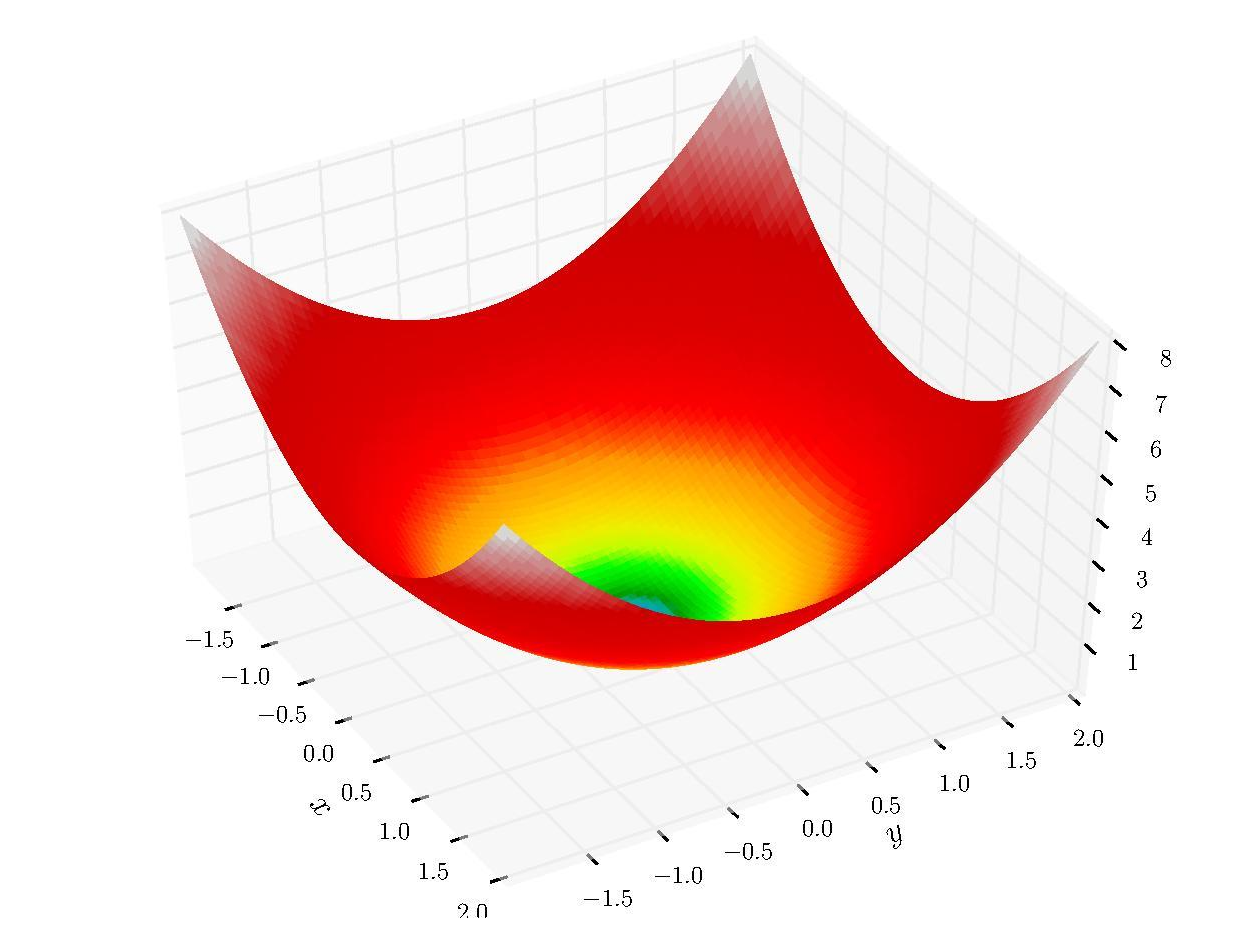
\includegraphics[width=0.9\textwidth]{sphere-function.eps}
\end{frame}

\begin{frame}{Sphere function}
	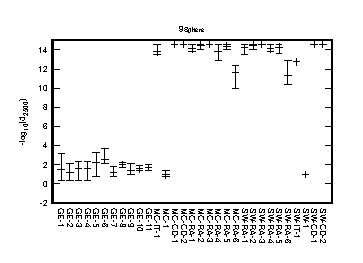
\includegraphics[width=\textwidth]{Sphere-e.eps}
\end{frame}

\begin{frame}{Ackley's function}
	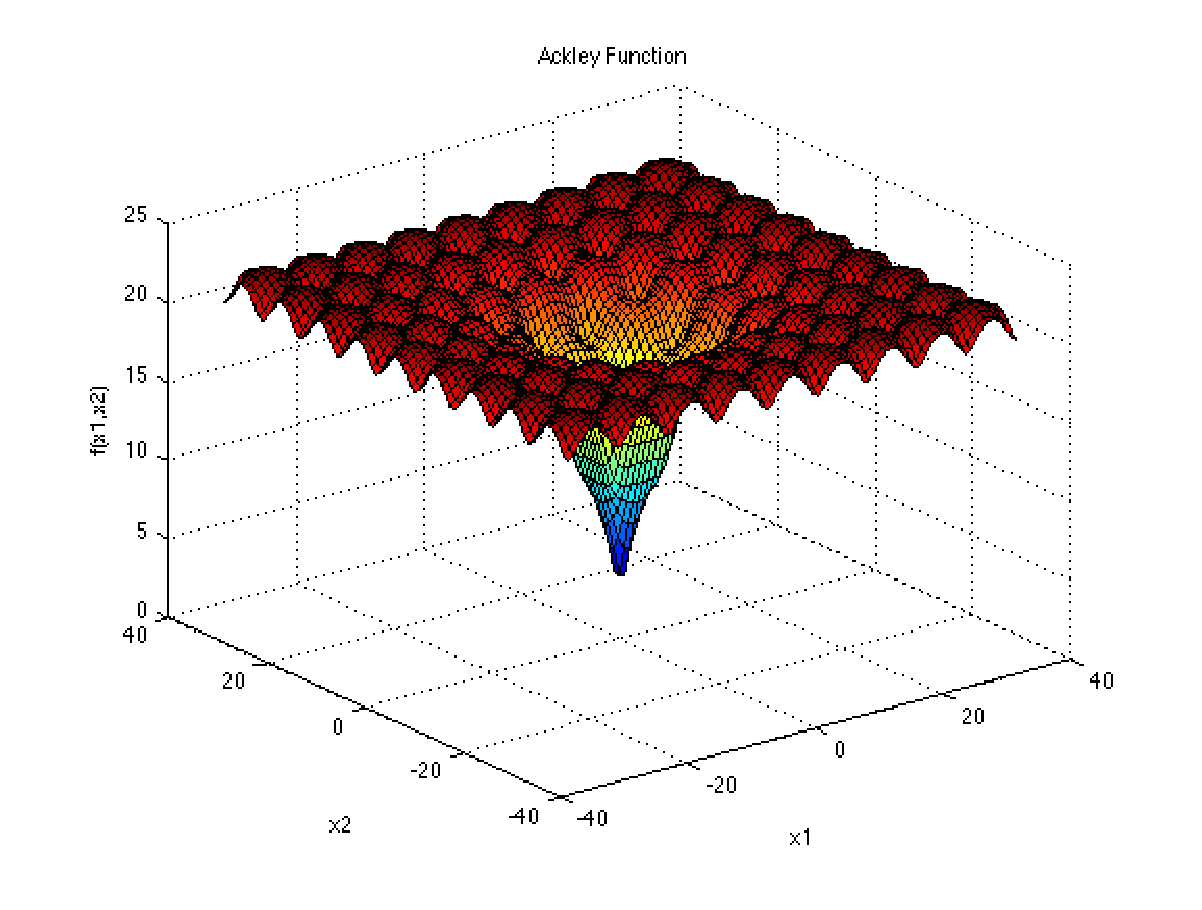
\includegraphics[width=0.9\textwidth]{ackley-function.eps}
\end{frame}

\begin{frame}{Ackley's function}
	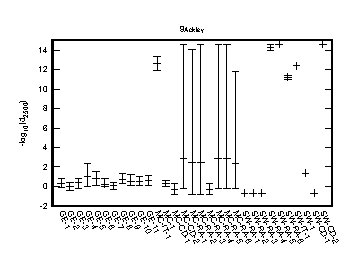
\includegraphics[width=\textwidth]{Ackley-e.eps}
\end{frame}

\begin{frame}{Booth's function}
	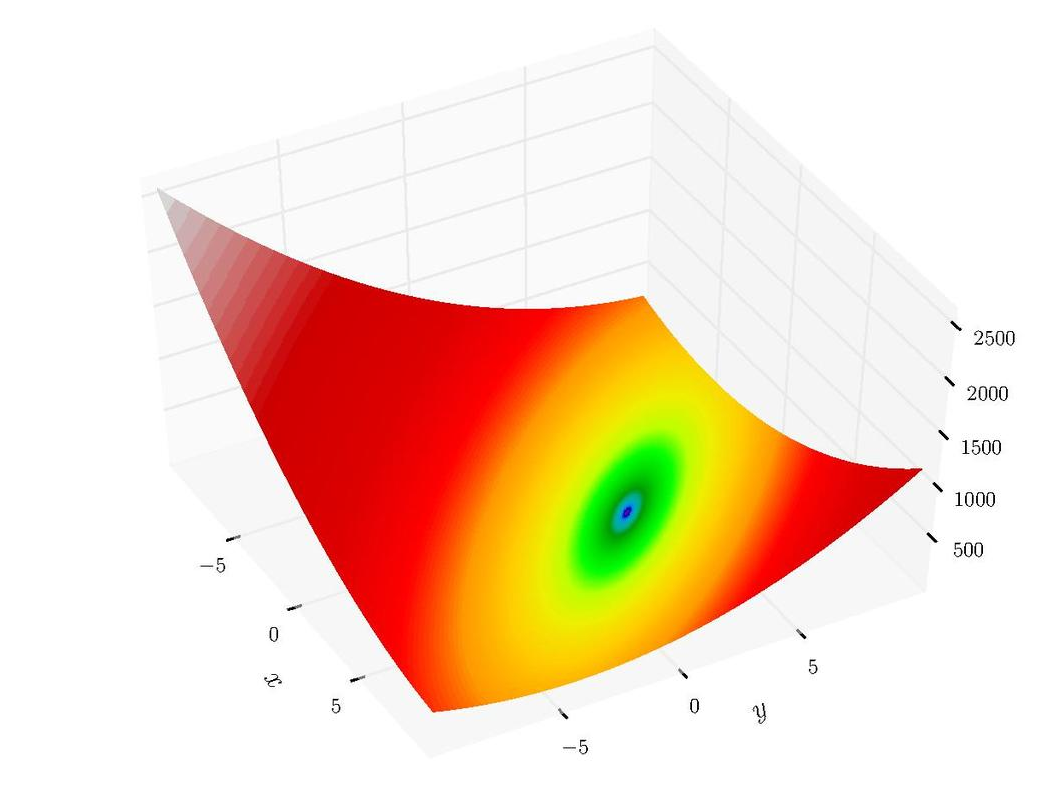
\includegraphics[width=0.9\textwidth]{booth-function.eps}
\end{frame}

\begin{frame}{Booth's function}
	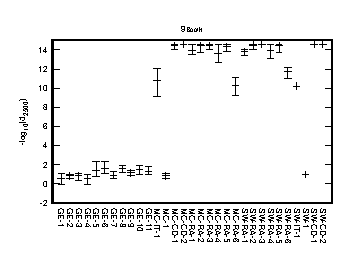
\includegraphics[width=\textwidth]{Booth-e.eps}
\end{frame}

\begin{frame}{Rosenbrock's function}
	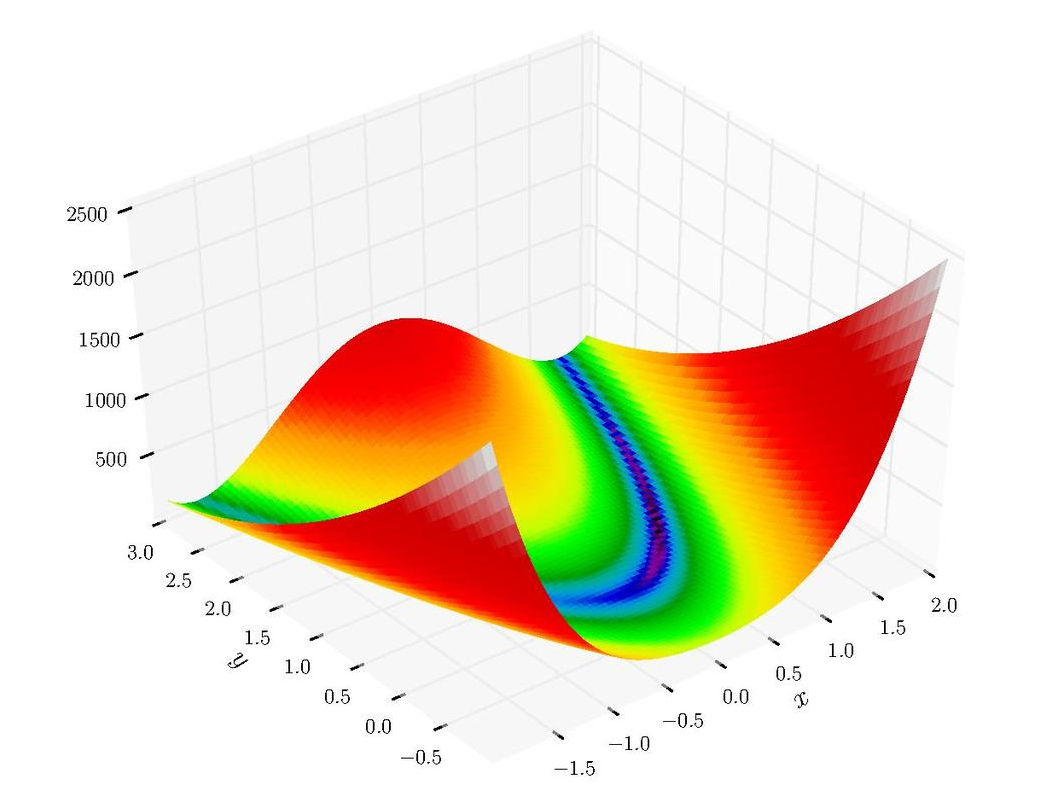
\includegraphics[width=0.9\textwidth]{rosenbrock-function.eps}
\end{frame}

\begin{frame}{Rosenbrock's function}
	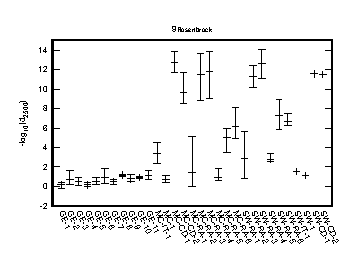
\includegraphics[width=\textwidth]{Rosenbrock-e.eps}
\end{frame}

\begin{frame}{Easom's function}
	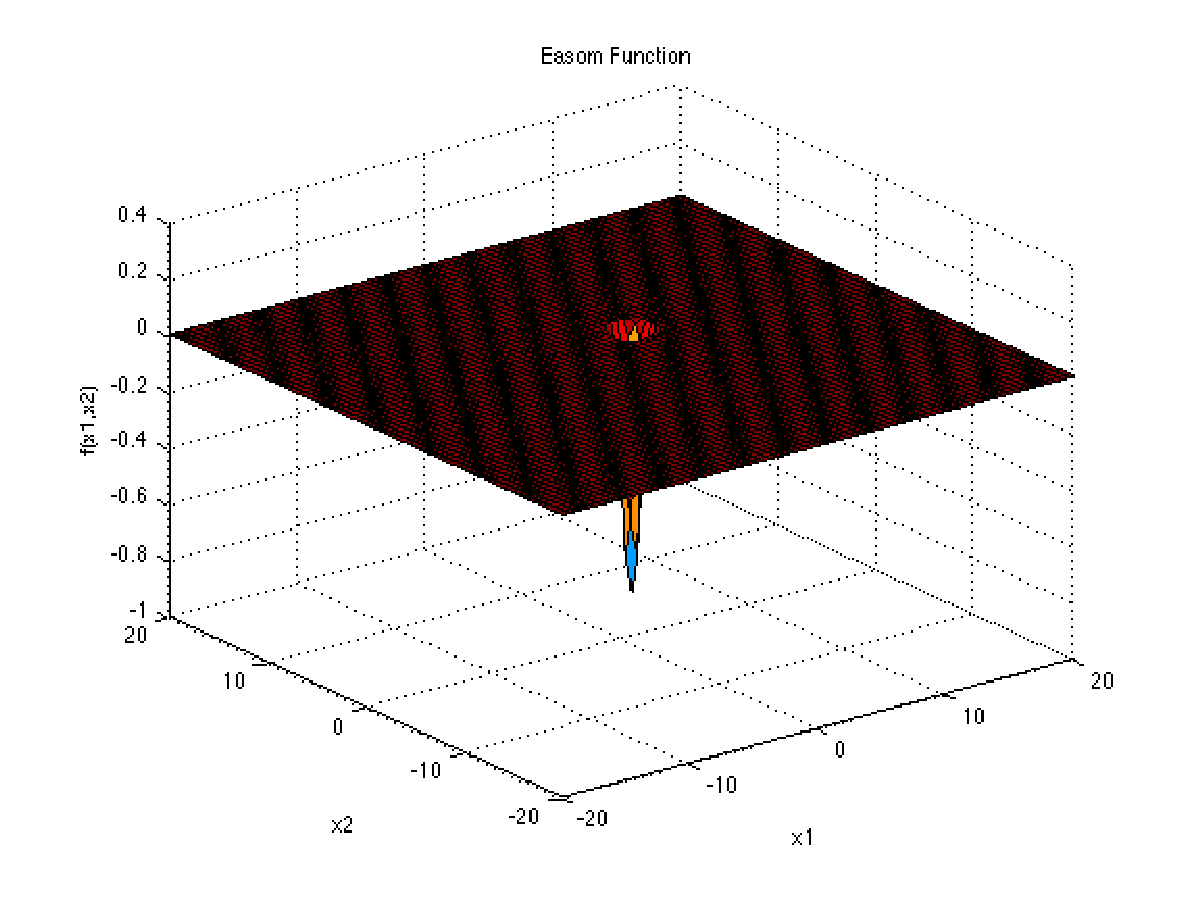
\includegraphics[width=0.9\textwidth]{easom-function.eps}
\end{frame}

\begin{frame}{Easom's function}
	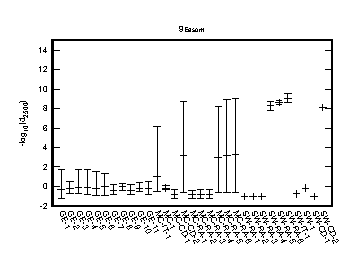
\includegraphics[width=\textwidth]{Easom-e.eps}
\end{frame}

\begin{frame}{Beale's function}
	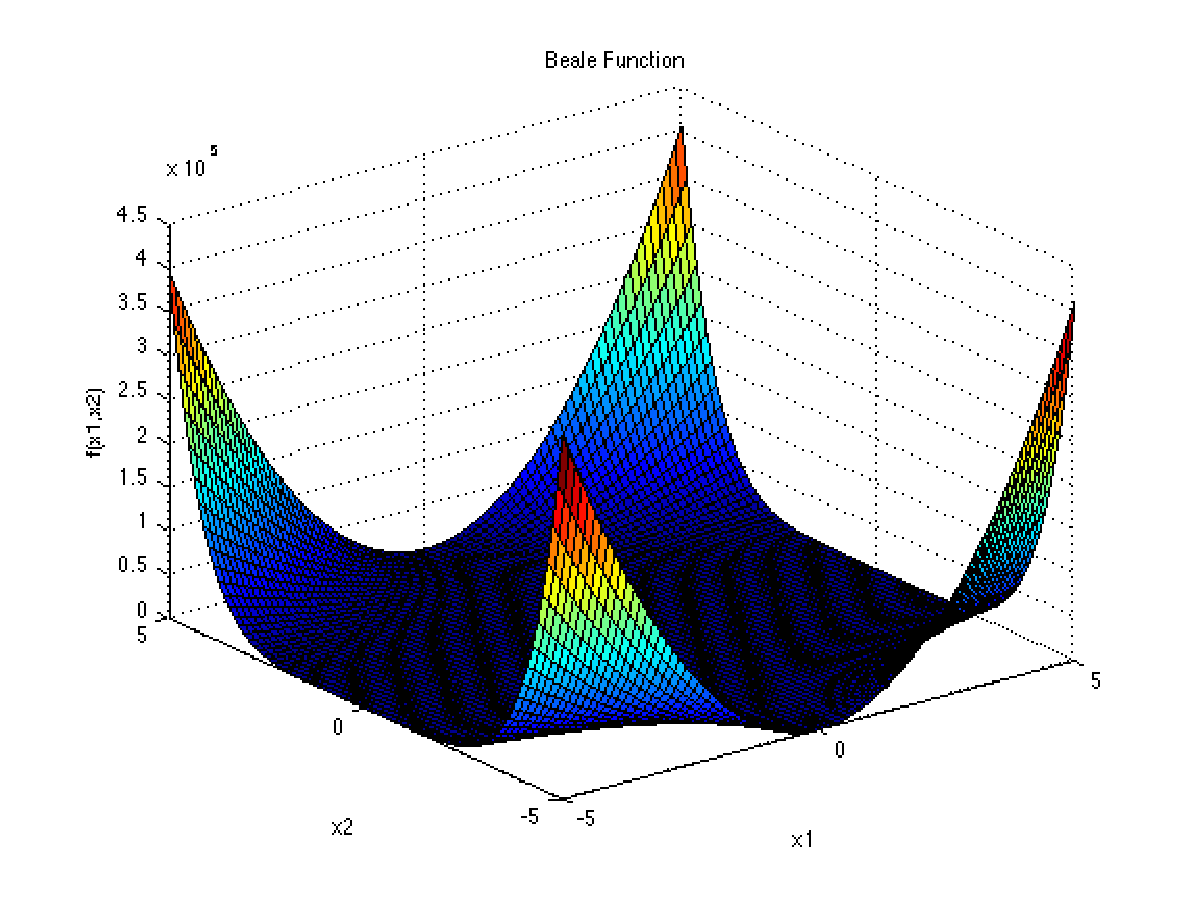
\includegraphics[width=0.9\textwidth]{beale-function.eps}
\end{frame}

\begin{frame}{Beale's function}
	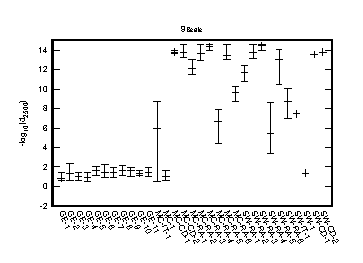
\includegraphics[width=\textwidth]{Beale-e.eps}
\end{frame}

\subsection{Parallelization}

\begin{frame}{Brute force algorithms: sweep and Monte-Carlo}
\psset{xunit=0.5mm,yunit=0.5mm}
\PSPICTURE{-90}{-55}{90}{-15}
{
	\tiny
	\rput(0,-15){Generation of $N_{total}$ empirical parameters sets}
	\psframe(-55,-20)(55,-10)
	\psline{->}(0,-20)(-50,-25)
	\psline{->}(0,-20)(0,-25)
	\psline{->}(0,-20)(55,-25)
	\rput(-55,-30){1st task:}
	\rput(-55,-35){$N_{total}/N_{tasks}$ simulations}
	\psframe(-90,-25)(-20,-40)
	\rput(0,-32.5){$\cdots$}
	\rput(55,-30){$N_{tasks}$-th task:}
	\rput(55,-35){$N_{total}/N_{tasks}$ simulations}
	\psframe(20,-25)(90,-40)
	\psline{->}(-55,-40)(0,-45)
	\psline{->}(0,-40)(0,-45)
	\psline{->}(55,-40)(0,-45)
	\rput(0,-50){Getting optimal empirical parameters set}
	\psframe(-50,-45)(50,-55)
}
\end{frame}

\begin{frame}{Iterative algorithm}
\psset{xunit=0.5mm,yunit=0.5mm}
\PSPICTURE{-100}{-130}{100}{-15}
{
	\tiny
	\rput(0,-15){1st iteration:}
	\rput(0,-20){Generation of $N_{simulations}$ empirical parameters sets}
	\psframe(-60,-25)(60,-10)
	\psline{->}(0,-25)(-60,-30)
	\psline{->}(0,-25)(0,-30)
	\psline{->}(0,-25)(60,-30)
	\rput(-60,-35){1st task:}
	\rput(-60,-40){$N_{simulations}/N_{tasks}$ simulations}
	\psframe(-100,-30)(-20,-45)
	\rput(0,-37.5){$\cdots$}
	\rput(60,-35){$N_{tasks}$-th task:}
	\rput(60,-40){$N_{simulations}/N_{tasks}$ simulations}
	\psframe(20,-30)(100,-45)
	\psline{->}(-60,-45)(0,-50)
	\psline{->}(0,-45)(0,-50)
	\psline{->}(60,-45)(0,-50)
	\rput(0,-55){Getting $N_{best}$ empirical parameters sets}
	\psframe(-55,-50)(55,-60)
	\psline{->}(0,-60)(0,-65)
	\rput(0,-70){$\cdots$}
	\psline{->}(0,-75)(0,-80)
	\rput(0,-85){$N_{iterations}$-th iteration:}
	\rput(0,-90){Generation of $N_{simulations}$ empirical parameters sets}
	\psframe(-60,-95)(60,-80)
	\psline{->}(0,-95)(-60,-100)
	\psline{->}(0,-95)(0,-100)
	\psline{->}(0,-95)(60,-100)
	\rput(-60,-105){1st task:}
	\rput(-60,-110){$N_{simulations}/N_{tasks}$ simulations}
	\psframe(-100,-100)(-20,-115)
	\rput(0,-107.5){$\cdots$}
	\rput(60,-105){$N_{tasks}$-th task:}
	\rput(60,-110){$N_{simulations}/N_{tasks}$ simulations}
	\psframe(20,-100)(100,-115)
	\psline{->}(-60,-115)(0,-120)
	\psline{->}(0,-115)(0,-120)
	\psline{->}(60,-115)(0,-120)
	\rput(0,-125){Getting optimal empirical parameters set}
	\psframe(-55,-120)(55,-130)
}
\end{frame}

\begin{frame}{Direction search algorithms}
\psset{xunit=0.5mm,yunit=0.5mm}
\PSPICTURE{-100}{-130}{100}{-15}
{
	\tiny
	\rput(0,-15){1st step:}
	\rput(0,-20){Generation of $N_{estimates}$ empirical parameters sets}
	\psframe(-60,-25)(60,-10)
	\psline{->}(0,-25)(-60,-30)
	\psline{->}(0,-25)(0,-30)
	\psline{->}(0,-25)(60,-30)
	\rput(-60,-35){1st task:}
	\rput(-60,-40){$N_{estimates}/N_{tasks}$ simulations}
	\psframe(-100,-30)(-20,-45)
	\rput(0,-37.5){$\cdots$}
	\rput(60,-35){$N_{tasks}$-th task:}
	\rput(60,-40){$N_{estimates}/N_{tasks}$ simulations}
	\psframe(20,-30)(100,-45)
	\psline{->}(-60,-45)(0,-50)
	\psline{->}(0,-45)(0,-50)
	\psline{->}(60,-45)(0,-50)
	\rput(0,-55){Getting optimal empirical parameters set}
	\psframe(-55,-50)(55,-60)
	\psline{->}(0,-60)(0,-65)
	\rput(0,-70){$\cdots$}
	\psline{->}(0,-75)(0,-80)
	\rput(0,-85){$N_{steps}$-th step:}
	\rput(0,-90){Generation of $N_{estimates}$ empirical parameters sets}
	\psframe(-60,-95)(60,-80)
	\psline{->}(0,-95)(-60,-100)
	\psline{->}(0,-95)(0,-100)
	\psline{->}(0,-95)(60,-100)
	\rput(-60,-105){1st task:}
	\rput(-60,-110){$N_{estimates}/N_{tasks}$ simulations}
	\psframe(-100,-100)(-20,-115)
	\rput(0,-107.5){$\cdots$}
	\rput(60,-105){$N_{tasks}$-th task:}
	\rput(60,-110){$N_{estimates}/N_{tasks}$ simulations}
	\psframe(20,-100)(100,-115)
	\psline{->}(-60,-115)(0,-120)
	\psline{->}(0,-115)(0,-120)
	\psline{->}(60,-115)(0,-120)
	\rput(0,-125){Getting optimal empirical parameters set}
	\psframe(-55,-120)(55,-130)
}
\end{frame}

\begin{frame}{Genetic}
\psset{xunit=0.4mm,yunit=0.4mm}
\PSPICTURE{-100}{-185}{100}{-15}
{
	\tiny
	\rput(0,-15){1st generation:}
	\rput(0,-20){Generation of $N_{population}$ empirical parameters sets}
	\psframe(-60,-25)(60,-10)
	\psline{->}(0,-25)(-60,-30)
	\psline{->}(0,-25)(0,-30)
	\psline{->}(0,-25)(60,-30)
	\rput(-60,-35){1st task:}
	\rput(-60,-40){$N_{population}/N_{tasks}$ simulations}
	\psframe(-100,-30)(-20,-45)
	\rput(0,-37.5){$\cdots$}
	\rput(60,-35){$N_{tasks}$-th task:}
	\rput(60,-40){$N_{population}/N_{tasks}$ simulations}
	\psframe(20,-30)(100,-45)
	\psline{->}(-60,-45)(0,-50)
	\psline{->}(0,-45)(0,-50)
	\psline{->}(60,-45)(0,-50)
	\rput(0,-55){Getting $N_{survival}$ empirical parameters sets}
	\psframe(-55,-50)(55,-60)
	\psline{->}(0,-60)(0,-65)
	\rput(0,-70){2nd generation:}
	\rput(0,-75){Generation of $N_{new}$ empirical parameters sets}
	\psframe(-55,-80)(55,-65)
	\psline{->}(0,-80)(-60,-85)
	\psline{->}(0,-80)(0,-85)
	\psline{->}(0,-80)(60,-85)
	\rput(-55,-90){1st task:}
	\rput(-55,-95){$N_{new}/N_{tasks}$ simulations}
	\psframe(-90,-85)(-20,-100)
	\rput(0,-92.5){$\cdots$}
	\rput(55,-90){$N_{tasks}$-th task:}
	\rput(55,-95){$N_{new}/N_{tasks}$ simulations}
	\psframe(20,-85)(90,-100)
	\psline{->}(-55,-100)(0,-105)
	\psline{->}(0,-100)(0,-105)
	\psline{->}(55,-100)(0,-105)
	\rput(0,-110){Getting $N_{survival}$ empirical parameters sets}
	\psframe(-55,-105)(55,-115)
	\psline{->}(0,-115)(0,-120)
	\rput(0,-125){$\cdots$}
	\psline{->}(0,-130)(0,-135)
	\rput(0,-140){$N_{generations}$-th generation:}
	\rput(0,-145){Generation of $N_{new}$ empirical parameters sets}
	\psframe(-55,-150)(55,-135)
	\psline{->}(0,-150)(-60,-155)
	\psline{->}(0,-150)(0,-155)
	\psline{->}(0,-150)(60,-155)
	\rput(-55,-160){1st task:}
	\rput(-55,-165){$N_{new}/N_{tasks}$ simulations}
	\psframe(-90,-155)(-20,-170)
	\rput(0,-162.5){$\cdots$}
	\rput(55,-160){$N_{tasks}$-th task:}
	\rput(55,-165){$N_{new}/N_{tasks}$ simulations}
	\psframe(20,-155)(90,-170)
	\psline{->}(-55,-170)(0,-175)
	\psline{->}(0,-170)(0,-175)
	\psline{->}(55,-170)(0,-175)
	\rput(0,-180){Getting optimal empirical parameters set}
	\psframe(-55,-175)(55,-185)
}
\end{frame}

\subsection{Convergence}

\begin{frame}{Iterative algorithm: best number and tolerance values}
	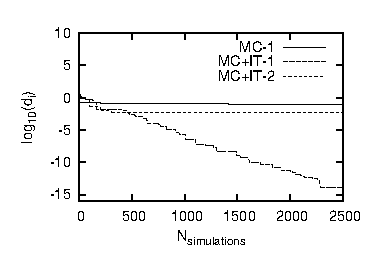
\includegraphics[width=0.9\textwidth]{sphere-evolution-mc.eps}
\end{frame}

\begin{frame}{Iterative algorithm: brute force simulations number}
	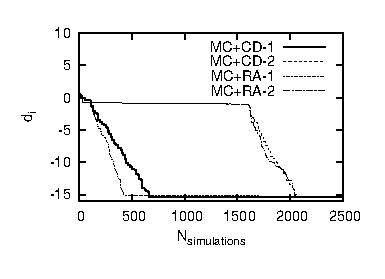
\includegraphics[width=0.9\textwidth]{sphere-evolution-mc-cdr.eps}
\end{frame}

\begin{frame}{Direction search algorithm: relaxation parameter}
	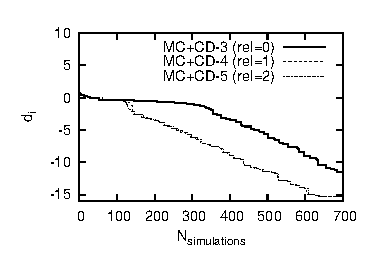
\includegraphics[width=0.9\textwidth]{sphere-evolution-mc-cd-r.eps}
\end{frame}

\begin{frame}{Direction search algorithm: step size}
	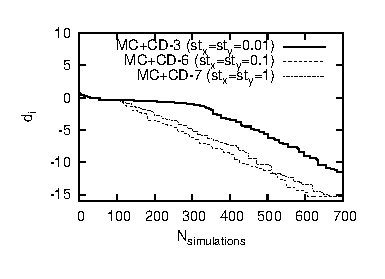
\includegraphics[width=0.9\textwidth]{sphere-evolution-mc-cd-s.eps}
\end{frame}

\begin{frame}{Random direction search algorithm: number of estimates}
	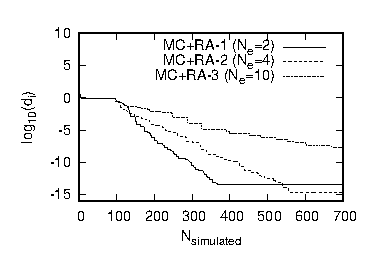
\includegraphics[width=0.9\textwidth]{sphere-evolution-mc-r.eps}
\end{frame}

\begin{frame}{Parallelization}
	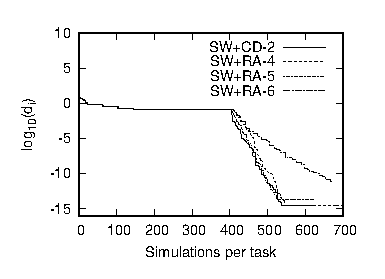
\includegraphics[width=0.49\textwidth]{sphere-task-2-4.eps}
	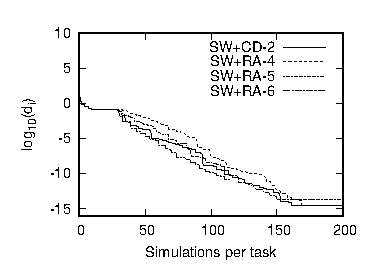
\includegraphics[width=0.49\textwidth]{sphere-task-2-64.eps}
\end{frame}

\section{MPCOTool}

\subsection{Organization}

\begin{frame}{Multi-Purposes Calibration and Optimization Tool}
\psset{xunit=0.35mm,yunit=0.35mm}
\PSPICTURE{-20}{-115}{260}{55}
{
	\tiny
	\rput(10,50){Main input file}
	\psframe(-20,45)(40,55)
	\psline{->}(40,50)(50,50)
	\rput(10,25){1st template file}
	\psframe(-20,20)(40,30)
	\psline{->}(40,25)(50,25)
	\psline[linestyle=dotted,dotsep=1pt]{->}(50,25)(90,25)
	\rput(10,15){$\cdots$}
	\rput(10,5){$n$-th template file}
	\psframe(-20,0)(40,10)
	\psline{->}(40,5)(50,5)
	\psline[linestyle=dotted,dotsep=1pt]{->}(50,5)(90,5)
	\rput(10,-35){$\cdots$}
	\rput(10,-75){$(N\,n)$-th template file}
	\psframe(-20,-70)(40,-80)
	\psline{->}(40,-75)(50,-75)
	\psline[linestyle=dotted,dotsep=1pt]{->}(50,-75)(90,-75)
	\rput(70,50){MPCOTool}
	\psframe(50,-95)(90,55)
	\rput(70,-110){Objective function value}
	\psframe(35,-105)(105,-115)
	\psline{->}(70,-95)(70,-105)
	\psline{->}(90,25)(100,25)
	\psline{->}(90,5)(100,5)
	\psline{->}(90,-55)(100,-55)
	\psline{->}(90,-75)(100,-75)
	\rput(120,5){$n$-th input file}
	\psframe(100,0)(140,10)
	\psline{->}(140,5)(150,5)
	\rput(120,15){$\cdots$}
	\rput(120,25){1st input file}
	\psframe(100,20)(140,30)
	\psline{->}(140,25)(145,25)(145,5)
	\rput(175,5){Simulator}
	\psframe(150,0)(200,10)
	\psline[linestyle=dashed,dash=2pt 1pt]{->}(175,10)(175,20)
	\psline[linestyle=dashed,dash=2pt 1pt]{->}(200,5)(210,7.5)
	\rput(175,25){Results file}
	\psframe[linestyle=dashed,dash=3pt 1pt](150,20)(200,30)
	\psline[linestyle=dashed,dash=2pt 1pt]{->}(200,25)(210,30)
	\rput(175,45){Experimental}
	\rput(175,40){data file}
	\psframe(150,35)(200,50)
	\psline[linestyle=dashed,dash=2pt 1pt]{->}(200,42.5)(210,30)
	\psline[linestyle=dashed,dash=2pt 1pt]{->}(150,42.5)(145,42.5)(145,25)
	\rput(230,30){Evaluator}
	\psline[linestyle=dashed,dash=2pt 1pt]{->}(230,25)(230,15)
	\psframe[linestyle=dashed,dash=3pt 1pt](210,25)(250,35)
	\rput(230,10){Objective}
	\rput(230,5){value file}
	\psframe(210,0)(250,15)
	\psline{->}(250,7.5)(260,7.5)(260,-90)(90,-90)
	\psline[linestyle=dotted,dotsep=1pt]{->}(90,-90)(70,-90)(70,-95)
	\rput(120,50){1st experiment}
	\psframe[linestyle=dotted](95,-5)(255,55)
	\rput(175,-15){$\cdots$}
	\rput(120,-75){$n$-th input file}
	\psframe(100,-80)(140,-70)
	\psline{->}(140,-75)(150,-75)
	\rput(120,-65){$\cdots$}
	\rput(120,-55){1st input file}
	\psframe(100,-60)(140,-50)
	\psline{->}(140,-55)(145,-55)(145,-75)
	\rput(175,-75){Simulator}
	\psframe(150,-80)(200,-70)
	\psline[linestyle=dashed,dash=2pt 1pt]{->}(175,-70)(175,-60)
	\psline[linestyle=dashed,dash=2pt 1pt]{->}(200,-75)(210,-72.5)
	\rput(175,-55){Results file}
	\psframe[linestyle=dashed,dash=3pt 1pt](150,-60)(200,-50)
	\psline[linestyle=dashed,dash=2pt 1pt]{->}(200,-55)(210,-50)
	\rput(175,-35){Experimental}
	\rput(175,-40){data file}
	\psframe(150,-30)(200,-45)
	\psline[linestyle=dashed,dash=2pt 1pt]{->}(200,-37.5)(210,-50)
	\psline[linestyle=dashed,dash=2pt 1pt]{->}(150,-37.5)(145,-37.5)(145,-55)
	\rput(230,-50){Evaluator}
	\psline[linestyle=dashed,dash=2pt 1pt]{->}(230,-55)(230,-65)
	\psframe[linestyle=dashed,dash=3pt 1pt](210,-55)(250,-45)
	\rput(230,-70){Objective}
	\rput(230,-75){value file}
	\psframe(210,-80)(250,-65)
	\psline(250,-72.5)(260,-72.5)
	\rput(120,-30){$N$-th experiment}
	\psframe[linestyle=dotted](95,-85)(255,-25)
}
\end{frame}

\subsection{Error norms}

\begin{frame}{Multi-Purposes Calibration and Optimization Tool}
	\[L_2:\quad J=\sqrt{\sum_{i=1}^{N_{exp}}\ABS{w_i\,o_i}^2},\]
	\[L_\infty:\quad J=\max_{i=1}^{N_{exp}}\ABS{w_i\,o_i},\]
	\[L_p:\quad J=\sqrt[p]{\sum_{i=1}^{N_{exp}}\ABS{w_i\,o_i}^p},\]
	\[L_1:\quad J=\sum_{i=1}^{N_{exp}}\ABS{w_i\,o_i},\]
\end{frame}

\begin{frame}{Main input file}
\psset{xunit=0.35mm,yunit=0.35mm}
\PSPICTURE{0}{-115}{280}{25}
{
	\tiny
	\psframe(0,-5)(280,25)
	\psline(40,-5)(40,25)
	\rput(20,20){\bf optimize}
	\rput(60,20){\bf simulator}
	\rput(95,20){\bf algorithm}
	\rput(130,20){evaluator}
	\rput(165,20){nsimulations}
	\rput(205,20){niterations}
	\rput(240,20){tolerance}
	\rput(265,20){nbest}
	\rput(60,10){threshold}
	\rput(95,10){npopulation}
	\rput(135,10){ngenerations}
	\rput(170,10){mutation}
	\rput(205,10){reproduction}
	\rput(240,10){adaptation}
	\rput(265,10){seed}
	\rput(60,0){direction}
	\rput(95,0){nsteps}
	\rput(130,0){nestimates}
	\rput(170,0){relaxation}
	\rput(200,0){norm}
	\rput(217,0){p}
	\rput(235,0){result}
	\rput(260,0){variables}
	\psline(20,-5)(20,-15)(40,-15)
	\psframe(40,-20)(280,-10)
	\psline(80,-20)(80,-10)
	\rput(60,-15){\bf experiment}
	\rput(95,-15){\bf name}
	\rput(125, -15){\bf template$_\mathbf{1}$}
	\rput(160,-15){template$_2$}
	\rput(195,-15){$\cdots$}
	\rput(230,-15){template$_n$}
	\rput(260,-15){weight}
	\psline(20,-15)(20,-25)
	\rput(140,-30){$\cdots$}
	\psline(20,-35)(20,-45)(40,-45)
	\psframe(40,-50)(280,-40)
	\psline(80,-50)(80,-40)
	\rput(60,-45){\bf experiment}
	\rput(95,-45){\bf name}
	\rput(125,-45){\bf template$_\mathbf{1}$}
	\rput(160,-45){template$_2$}
	\rput(195,-45){$\cdots$}
	\rput(230,-45){template$_n$}
	\rput(260,-45){weight}
	\psline(20,-45)(20,-65)(40,-65)
	\psframe(40,-75)(280,-55)
	\psline(80,-75)(80,-55)
	\rput(60,-60){\bf variable}
	\rput(95,-60){\bf name}
	\rput(120,-60){\bf minimum}
	\rput(152.5,-60){\bf maximum}
	\rput(195,-60){absolute\_minimum}
	\rput(250,-60){absolute\_maximum}
	\rput(100,-70){precision}
	\rput(130,-70){nsweeps}
	\rput(155,-70){nbits}
	\rput(175,-70){step}
	\psline(20,-65)(20,-80)
	\rput(140,-85){$\cdots$}
	\psline(20,-90)(20,-105)(40,-105)
	\psframe(40,-115)(280,-95)
	\psline(80,-115)(80,-95)
	\rput(60,-100){\bf variable}
	\rput(95,-100){\bf name}
	\rput(120,-100){\bf minimum}
	\rput(152.5,-100){\bf maximum}
	\rput(195,-100){absolute\_minimum}
	\rput(250,-100){absolute\_maximum}
	\rput(100,-110){precision}
	\rput(130,-110){nsweeps}
	\rput(155,-110){nbits}
	\rput(175,-110){step}
}
\end{frame}

\defverbatim[colored]\makeseti{
\lstset{
  language=xml,
  extendedchars=true,
  basicstyle=\tiny\ttfamily,
  showstringspaces=false,
  showspaces=false,
  tabsize=4,
  breaklines=true,
  showtabs=false,
  captionpos=b
  keywordstyle=\color{blue}\ttfamily,
  stringstyle=\color{red}\ttfamily,
}
\begin{lstlisting}[language=xml]
<optimize simulator="simulator_name" evaluator="evaluator_name"
	algorithm="algorithm_type" nsimulations="simulations_number"
	niterations="iterations_number" tolerance="tolerance_value"
	nbest="best_number" npopulation="population_number"
	ngenerations="generations_number" mutation="mutation_ratio"
	reproduction="reproduction_ratio" adaptation="adaptation_ratio"
	direction="direction_search_type" nsteps="steps_number"
	relaxation="relaxation_parameter" nestimates="estimates_number"
	threshold="threshold_parameter" norm="norm_type" p="p_parameter"
	seed="random_seed" result_file="result_file"
	variables_file="variables_file">
    <experiment name="data_file_1" template1="template_1_1"
		template2="template_1_2" ... weight="weight_1"/>
    ...
    <experiment name="data_file_N" template1="template_N_1"
		template2="template_N_2" ... weight="weight_N"/>
    <variable name="variable_1" minimum="min_value" maximum="max_value"
		precision="precision_digits" sweeps="sweeps_number"
		nbits="bits_number" step="step_size"/>
    ...
    <variable name="variable_M" minimum="min_value" maximum="max_value"
		precision="precision_digits" sweeps="sweeps_number"
		nbits="bits_number" step="step_size"/>
</optimize>
\end{lstlisting}
}

\subsection{Input files}

\begin{frame}{Main input file: XML format}
	\makeseti
\end{frame}

\defverbatim[colored]\makesetii{
\lstset{
  language=json,
  extendedchars=true,
  basicstyle=\tiny\ttfamily,
  showstringspaces=false,
  showspaces=false,
  tabsize=4,
  breaklines=true,
  showtabs=false,
  captionpos=b
  keywordstyle=\color{green}\ttfamily,
  stringstyle=\color{red}\ttfamily,
}
\begin{lstlisting}[language=json,multicols=2]
{
	"simulator": "simulator_name",
	"evaluator": "evaluator_name",
	"algorithm": "algorithm_type",
	"nsimulations": "simulations_number",
	"niterations": "iterations_number",
	"tolerance": "tolerance_value",
	"nbest": "best_number",
	"npopulation": "population_number",
	"ngenerations": "generations_number",
	"mutation": "mutation_ratio",
	"reproduction": "reproduction_ratio",
	"adaptation": "adaptation_ratio",
	"direction": "direction_search_type",
	"nsteps": "steps_number",
	"relaxation": "relaxation_parameter",
	"nestimates": "estimates_number",
	"threshold": "threshold_parameter",
	"norm": "norm_type",
	"p": "p_parameter",
	"seed": "random_seed",
	"result_file": "result_file",
	"variables_file": "variables_file",
	"experiments":
	[
		{
			"name": "data_file_1",
			"template1": "template_1_1",
			"template2": "template_1_2",
			...
			"weight": "weight_1",
		},
	    ...
		{
			"name": "data_file_N",
			"template1": "template_N_1",
			"template2": "template_N_2",
			...
			"weight": "weight_N",
		}
	],
	"variables":
	[
		{

			"name": "variable_1",
			"minimum": "min_value",
			"maximum": "max_value",
			"precision": "precision_digits",
			"sweeps": "sweeps_number",
			"nbits": "bits_number",
			"step": "step_size",
		},
		...
		{
			"name": "variable_M",
			"minimum": "min_value",
			"maximum": "max_value",
			"precision": "precision_digits",
			"sweeps": "sweeps_number",
			"nbits": "bits_number",
			"step": "step_size",
		}
	]
}
\end{lstlisting}
}

\begin{frame}{Main input file: JSON format}
	\makesetii
\end{frame}

\begin{frame}{Template files}
	\begin{itemize}
		\item $N_{experiments}\times N_{inputs}$ template files are required
		\item MPCOTool parses the templates to generate the input files for
			every simulation:
		\begin{itemize}
			\item[@variableX@]: is replaced by the label associated to the
				$X$-th parameter
			\item[@valueX@]: is replaced by the value associated to the $X$-th
				parameter calculated by the optimization algorithm using the
				main input file data
		\end{itemize}
	\end{itemize}
\end{frame}

\subsection{User instructions}

\begin{frame}{MPCOTool: building}
	\begin{itemize}
		\item Free software, BSD type license.
		\item Repository \url{https://github.com/jburguete/mpcotool}
		\item Code in C
		\item Tools required to build the executable
			\begin{itemize}
				\item C compiler: GCC or CLang
				\item Configuration tools: Automake, Autoconf and PKGConfig
				\item Control tool: GNUMake
			\end{itemize}
	\end{itemize}
\end{frame}

\begin{frame}{MPCOTool: building}
	\begin{itemize}
		\item Free software, BSD type license.
		\item Repository \url{https://github.com/jburguete/mpcotool}
		\item Code in C
		\item Tools required to build the executable
		\item Free external libraries
		\begin{itemize}
			\item Libxml2: main input file in XML format
			\item JSON-GLib: main input file in JSON format
			\item GSL: to generate pseudo-random numbers
			\item GLib: to parse input templates and to parallelize in the CPU
				cores
			\item Gettext: to work with different international languages
			\item GTK+3: interactive graphic interface (optional)
			\item OpenMPI or MPICH: to parallelize in computer clusters
				(optional)
		\end{itemize}
	\end{itemize}
\end{frame}

\begin{frame}{MPCOTool: building}
	\begin{itemize}
		\item Free software, BSD type license.
		\item Repository \url{https://github.com/jburguete/mpcotool}
		\item Code in C
		\item Tools required to build the executable
		\item Free external libraries
		\item Multiplatform
		\begin{itemize}
			\item Linux (Debian, Ubuntu, Fedora, OpenSUSE, Mint)
			\item Microsoft Windows (7, 8.1, 10)
			\item BSD (FreeBSD, OpenBSD, NetBSD, DragonflyBSD, Debian kFreeBSD)
			\item Illumos (Dyson, OpenIndiana)
			\item Hurd (Debian)
		\end{itemize}
	\end{itemize}
\end{frame}

\begin{frame}{MPCOTool: building}
	\begin{itemize}
		\item Free software, BSD type license.
		\item Repository \url{https://github.com/jburguete/mpcotool}
		\item Code in C
		\item Tools required to build the executable
		\item Free external libraries
		\item Multiplatform
		\item Languages
		\begin{itemize}
			\item English
			\item Spanish
			\item French
			\item German
		\end{itemize}
	\end{itemize}
\end{frame}

\begin{frame}{MPCOTool: command line}
	\begin{itemize}
		\item Running in one computer
	\end{itemize}
.$/$mpcotoolbin [-nthreads X] [-seed S] main\_input\_file.xml [results\_file]
[variables\_file]
	\begin{itemize}
		\item Parallelization in computers cluster with MPI
	\end{itemize}
mpirun [MPI options] .$/$mpcotoolbin [-nthreads X] [-seed S]
main\_input\_file.xml [results\_file] [variables\_file]
	\begin{itemize}
		\item Simulation program syntax
	\end{itemize}
.$/$simulator input\_file\_1 [input\_file\_2] [...] output\_file
	\begin{itemize}
		\item Evaluation program syntax (optional)
	\end{itemize}
.$/$evaluator simulated\_file experiment\_file results\_file
\end{frame}

\begin{frame}{MPCOTool: graphic user interface application}
	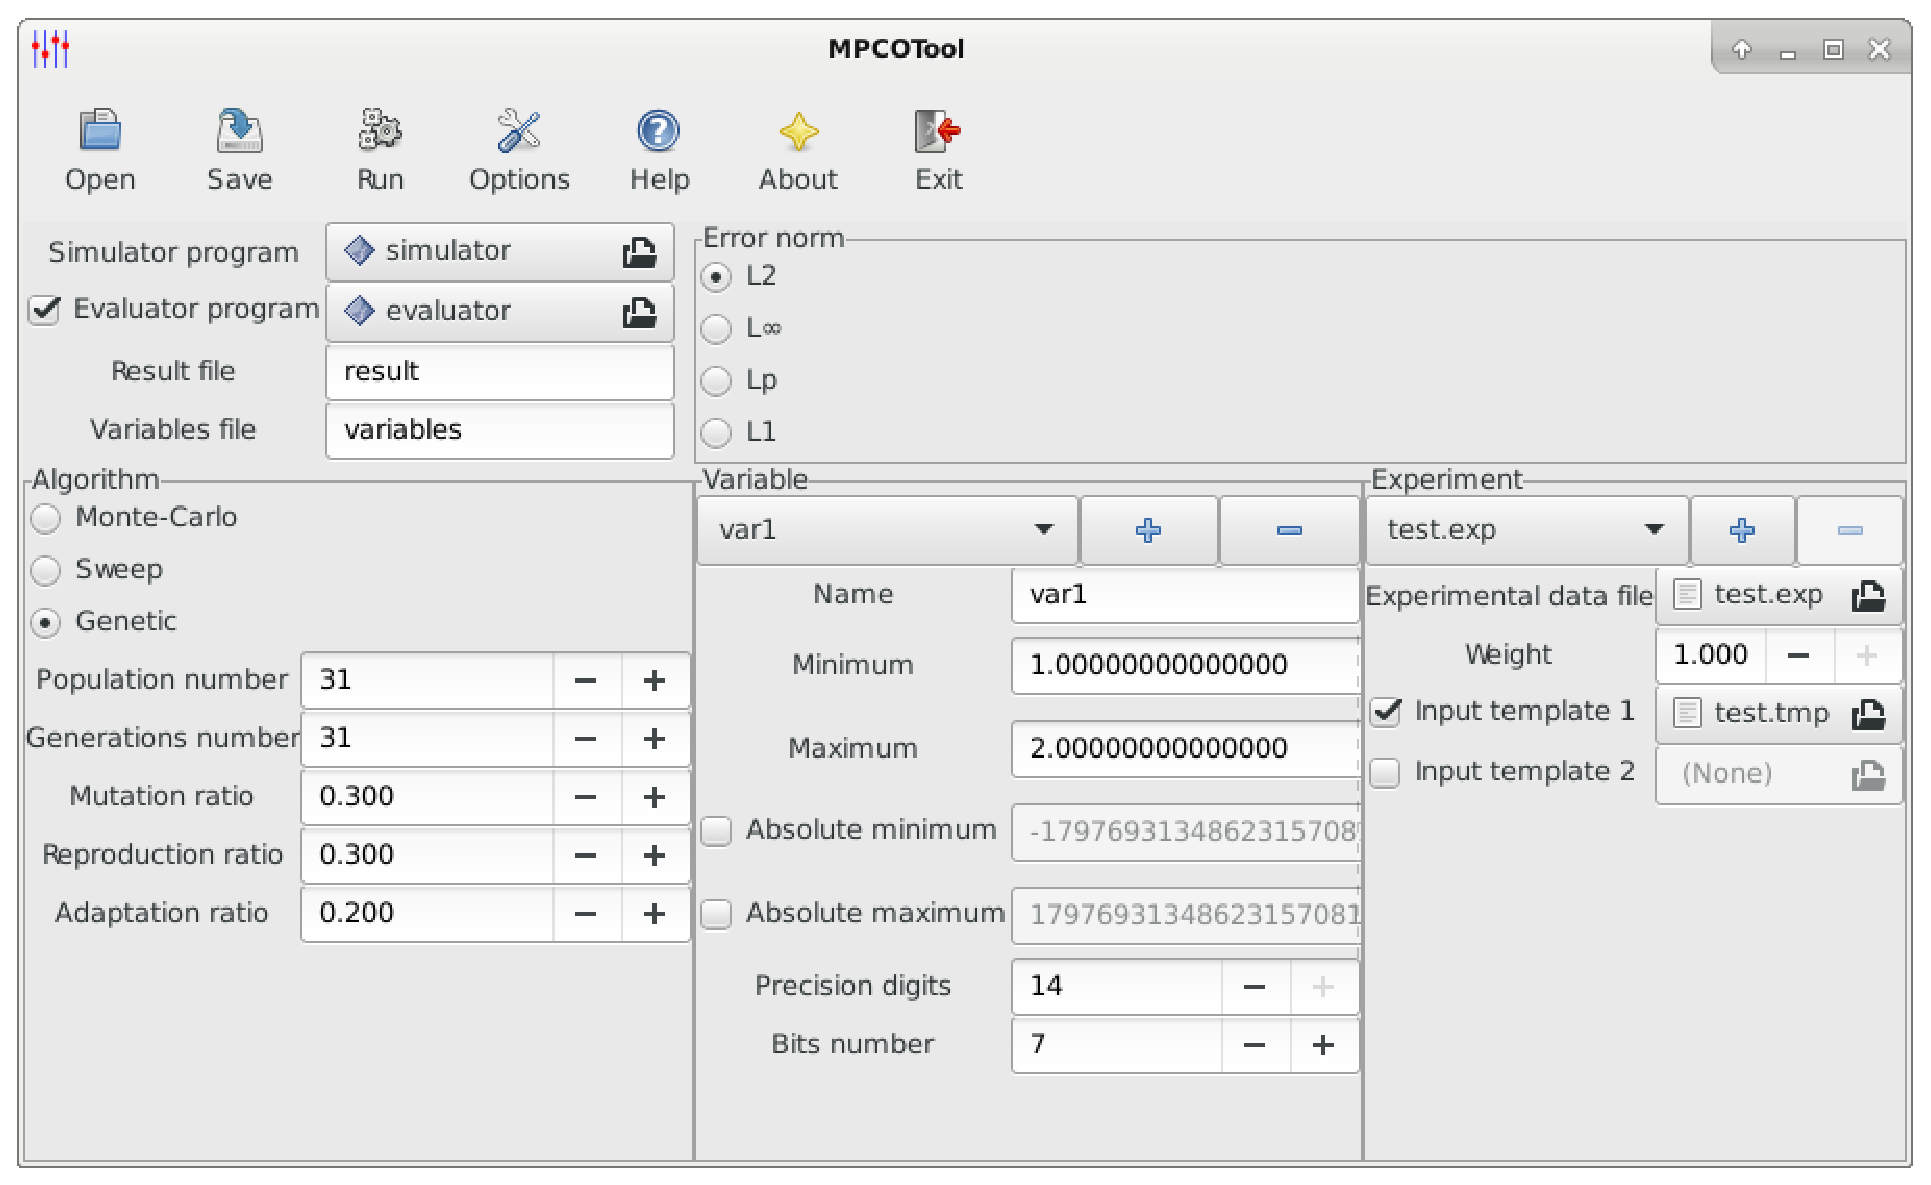
\includegraphics[width=\textwidth]{mpcotool-en.eps}
\end{frame}

\begin{frame}{MPCOTool: output files}
	\begin{itemize}
		\item Results: optimal objective function and variable values, and
			calculation time
		\item Variables: all objective function and variable values tried by the
			optimization algorithm
	\end{itemize}
\end{frame}

\section{Practical applications}

\subsection{Optimization of gate times in a canal}

\begin{frame}{Canal ``La Violada''}
	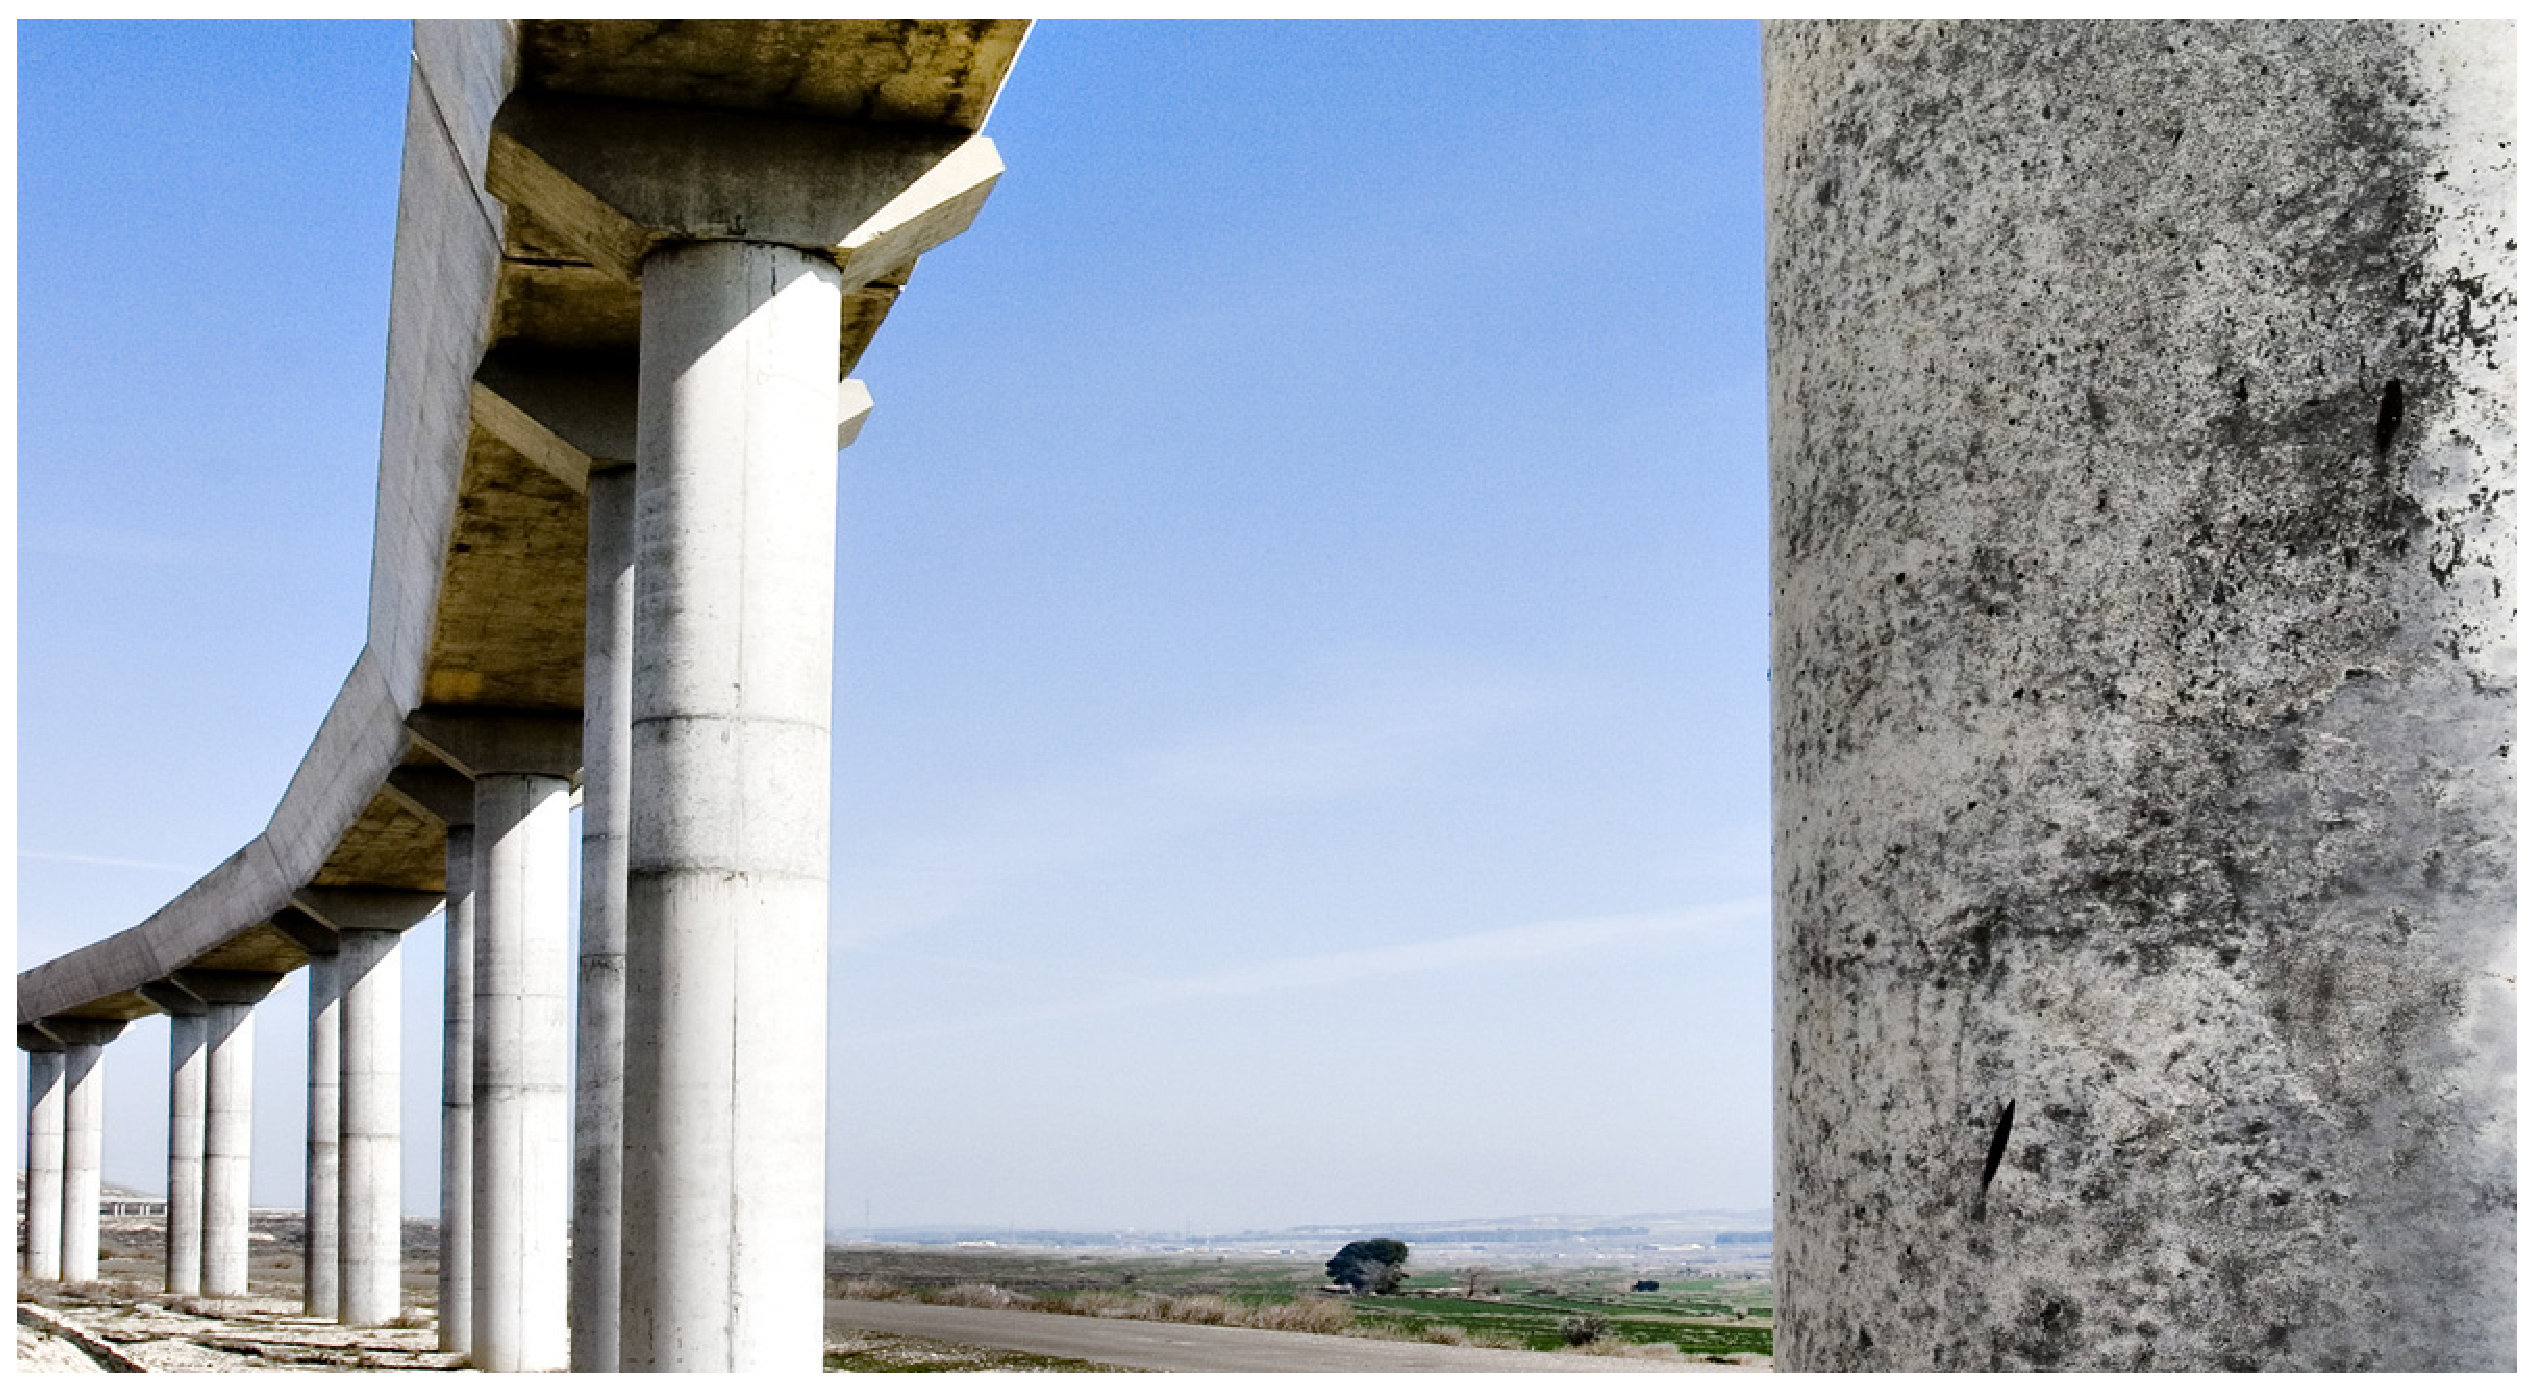
\includegraphics[width=\textwidth]{CanalLaViolada.eps}
\end{frame}

\begin{frame}{Canal ``La Violada''}
\psset{xunit=8mm,yunit=5mm}
\PSPICTURE{-1}{-2}{11.4}{2}
{
	\scriptsize
	\rput(-0.5,0){Inlet}
	\rput(10.7,0){Outlet}
	\psline(0,0)(10,0)
	\psline{->}(7.5,0)(7.5,-1)
	\rput(7.5,-1.4){Spillway}
	\psline{->}(10,0)(10,-1)
	\rput(10,-1.4){Spillway}
	\psline{->}(3,0)(3,1)
	\rput(3,1.4){Almudévar}
	\psline{->}(8.5,0)(7.5,1)
	\rput(7.5,1.4){Gurrea}
	\psline{->}(9,0)(10,1)
	\rput(10,1.4){El Temple}
	\psline{<->}(0,-0.3)(3,-0.3)
	\rput(1.5,-0.7){5007 m}
	\psline{<->}(3,-0.3)(7.5,-0.3)
	\rput(5.25,-0.7){8346 m}
	\psline{<->}(7.5,-0.3)(8.5,-0.3)
	\rput(8,-0.7){270 m}
	\psline{<->}(8.5,-0.3)(9,-0.3)
	\rput(8.75,-0.7){7 m}
	\psline{<->}(9,-0.3)(10,-0.3)
	\rput(9.5,-0.7){27 m}
}
\psset{xunit=8mm,yunit=8mm}
\PSPICTURE{0}{-0.6}{12.7}{2.450}
{
	\scriptsize
	\psline(0,2.050)(0.615,0)(3.259,0)(3.874,2.050)
	\psline{<->}(0.615,-0.2)(3.259,-0.2)
	\rput(1.937,-0.4){2.644 m}
	\psline{<->}(0,2.250)(3.874,2.250)
	\rput(1.937,2.450){3.874 m}
	\psline{<->}(4.074,0)(4.074,2.050)
	\rput(4.774,1.025){2.050 m}
	\psline(5.5,1.8)(5.5,1.5)(7,0)(9.5,0)(11,1.5)(11,1.8)
	\psline{<->}(5.5,2)(11,2)
	\rput(8.25,2.2){5.500 m}
	\psline{<->}(7,-0.2)(9.5,-0.2)
	\rput(8.25,-0.4){2.500 m}
	\psline{<->}(11.2,0)(11.2,1.5)
	\rput(11.9,0.75){1.500 m}
	\psline{<->}(11.2,1.5)(11.2,1.8)
	\rput(11.95,1.65){0.300 m}
}
\end{frame}

\begin{frame}{Canal ``La Violada''}
	\framesubtitle{Optimization}
	\begin{itemize}
		\item 15 days of simulation
		\item 1024 simulations
		\item $\approx$ 14-19h using 64 cores in the Memento cluster from the BIFI
	\end{itemize}
\end{frame}

\begin{frame}{Canal ``La Violada''}
\TABLE{\tiny}{cccc}
{
	Optimization & Optimization & Optimal empirical & Objective
	\\ algorithm & parameters & parameters & function value
	\\ \hline
	\multicolumn{2}{c}{Manual management} & $\Delta t_A=3600$ s
	& 1.049056 m$^6$/s$^2$
	\\ & & $\Delta t_{GT}=12600$ s
	\\ \hline
	SW & $N_{\Delta t_A}=N_{\Delta t_{GT}}=32$ & $\Delta t_A=3368$ s
	& 0.047170 m$^6$/s$^2$
	\\ & & $\Delta t_{GT}=3716$ s
	\\ \hline
	SW+IT & $N_{\Delta t_A}=N_{\Delta t_{GT}}=16$ & $\Delta t_A=3266$ s
	& 0.047413 m$^6$/s$^2$
	\\ & $N_i=4$, $N_b=4$, $tol=0.5$ & $\Delta t_{GT}=3840$ s
	\\ \hline
	MC & $N_s=1024$ & $\Delta t_A=3193$ s & 0.047183 m$^6$/s$^2$
	\\ & & $\Delta t_{GT}=3705$ s
	\\ \hline
	MC+IT & $N_s=256$ & $\Delta t_A=3250$ s & 0.047139 m$^6$/s$^2$
	\\ & $N_i=N_b=4$, $tol=0.1$ & $\Delta t_{GT}=3751$ s
	\\ \hline
	MC+DS+RA & $N_s=768$, $N_{st}=4$ & $\Delta t_A=3211$ s
		& 0.047129 m$^6$/s$^2$
	\\ & $N_e=64$, $rel=1$ & $\Delta t_{GT}=3754$ s
	\\ & $st_{\Delta t_A}=st_{\Delta t_{GT}}=10$ s 
	\\ \hline
	GE & $N_p=256$, $N_g=9$ & $\Delta t_A=3274$ s & 0.047134 m$^6$/s$^2$
	\\ & $R_m=R_r=R_a=0.125$ & $\Delta t_{GT}=3753$ s
	\\ \hline
	GE & $N_p=64$, $N_g=21$ & $\Delta t_A=3338$ s & 0.047150 m$^6$/s$^2$
	\\ & $R_m=R_r=R_a=0.25$ & $\Delta t_{GT}=3740$ s
	\\ \hline
}
\end{frame}

\begin{frame}{Canal ``La Violada''}
	\framesubtitle{Direction search algorithm: parallelization}
	\begin{itemize}
		\item Monte-Carlo: 768 simulations, 12 per core, $\approx 60.3$ active cores
		\item Random direction search: 64 estimates, 1 per core, 4 iterations
			$\approx 41.2$ active cores
	\end{itemize}
	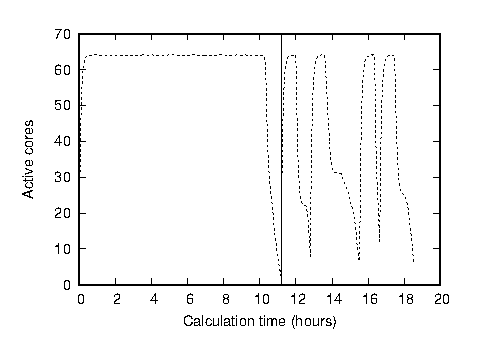
\includegraphics[width=0.8\textwidth]{load-swigs-mc-ra-768-1-64-4.eps}
\end{frame}

\begin{frame}{Canal ``La Violada''}
	\framesubtitle{Manual management}
	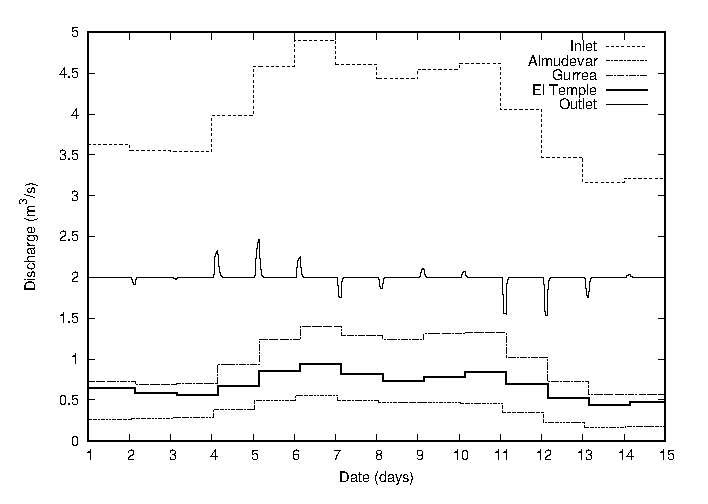
\includegraphics[width=0.9\textwidth]{Violada-contributions.eps}
\end{frame}

\begin{frame}{Canal ``La Violada''}
	\framesubtitle{Optimal management}
	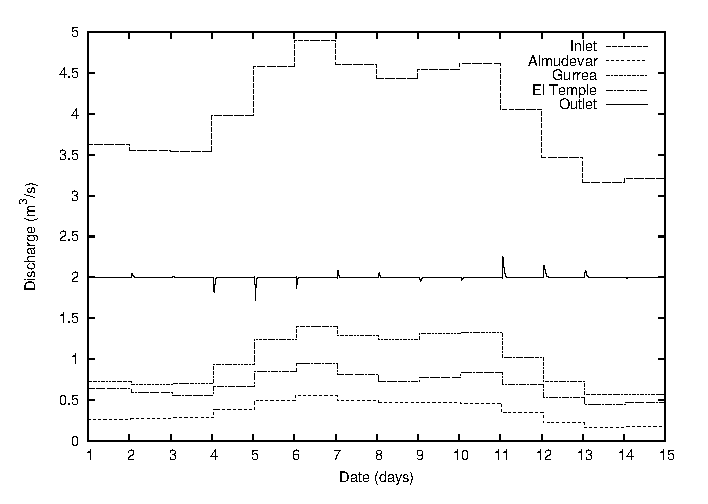
\includegraphics[width=0.9\textwidth]{Violada-optimized-contributions.eps}
\end{frame}

\subsection{Calibration of roughness and infiltration
coefficients in furrows}

\begin{frame}{Furrow irrigation}
\psset{xunit=13mm,yunit=13mm}
\PSPICTURE{-0.7}{-0.4}{6.5}{2.45}
{
	\scriptsize
	\psline(0,0.27)(0.2,0.27)(0.53,0)(0.67,0)
		(1,0.27)(1.2,0.27)(1.53,0)(1.67,0)
		(2,0.27)(2.2,0.27)(2.53,0)(2.67,0)
		(3,0.27)(3.2,0.27)(3.53,0)(3.67,0)(4,0.27)(4.2,0.27)
	\psline(0,0.27)(2,2.27)
	\psline(0.2,0.27)(2.2,2.27)
	\psline(0.53,0)(2.53,2)
	\psline(0.67,0)(2.67,2)
	\psline(1,0.27)(3,2.27)
	\psline(1.2,0.27)(3.2,2.27)
	\psline(1.53,0)(3.53,2)
	\psline(1.67,0)(3.67,2)
	\psline(2,0.27)(4,2.27)
	\psline(2.2,0.27)(4.2,2.27)
	\psline(2.53,0)(4.53,2)
	\psline(2.67,0)(4.67,2)
	\psline(3,0.27)(5,2.27)
	\psline(3.2,0.27)(5.2,2.27)
	\psline(3.53,0)(5.53,2)
	\psline(3.67,0)(5.67,2)
	\psline(4,0.27)(6,2.27)
	\psline(4.2,0.27)(6.2,2.27)
	\psline(2,2.27)(2.2,2.27)(2.53,2)(2.67,2)
		(3,2.27)(3.2,2.27)(3.53,2)(3.67,2)
		(4,2.27)(4.2,2.27)(4.53,2)(4.67,2)
		(5,2.27)(5.2,2.27)(5.53,2)(5.67,2)(6,2.27)(6.2,2.27)
	\psline[linestyle=dashed, dash=2pt 1pt](0,0.27)(-0.2,0.27)
	\psline[linestyle=dashed, dash=2pt 1pt](0.53,0)(-0.2,0)
	\psline{<->}(-0.1,0.27)(-0.1,0)
	\rput(-0.4,0.135){0.27m}
	\psline[linestyle=dashed, dash=2pt 1pt](2,2.27)(1.8,2.27)
	\psline{<->}(-0.1,0.27)(1.9,2.27)
	\rput(0.6,1.27){100m}
	\psline[linestyle=dashed, dash=2pt 1pt](0.53,0)(0.53,-0.2)
	\psline[linestyle=dashed, dash=2pt 1pt](0.67,0)(0.67,-0.2)
	\psline{->}(0.43,-0.1)(0.53,-0.1)
	\psline{->}(0.77,-0.1)(0.67,-0.1)
	\rput(0.6,-0.3){0.14m}
	\psline[linestyle=dashed, dash=2pt 1pt](1.2,0.27)(1.2,-0.2)
	\psline[linestyle=dashed, dash=2pt 1pt](2,0.27)(2,-0.2)
	\psline{<->}(1.2,-0.1)(2,-0.1)
	\rput(1.6,-0.3){0.80m}
	\psline[linestyle=dashed, dash=2pt 1pt](2.2,0.27)(2.2,-0.2)
	\psline{<->}(2,-0.1)(2.2,-0.1)
	\rput(2.1,-0.3){0.20m}
	\psline[linestyle=dashed, dash=2pt 1pt](4.2,0.27)(4.4,0.27)
	\psline[linestyle=dashed, dash=2pt 1pt](0.4,0.67)(4.8,0.67)
	\psline{<->}(4.3,0.27)(4.7,0.67)
	\rput(4.8,0.47){20m}
	\rput(5,0.67){S20}
	\psline[linestyle=dashed, dash=2pt 1pt](0.8,1.07)(5.2,1.07)
	\psline{<->}(4.7,0.67)(5.1,1.07)
	\rput(5.2,0.87){20m}
	\rput(5.4,1.07){S40}
	\psline[linestyle=dashed, dash=2pt 1pt](1.2,1.47)(5.6,1.47)
	\psline{<->}(5.1,1.07)(5.5,1.47)
	\rput(5.6,1.27){20m}
	\rput(5.8,1.47){S60}
	\psline[linestyle=dashed, dash=2pt 1pt](1.6,1.87)(6,1.87)
	\psline{<->}(5.5,1.47)(5.9,1.87)
	\rput(6,1.67){20m}
	\rput(6.2,1.87){S80}
	\rput(2.6,2.3){Q1}
	\rput(3.6,2.3){Q2}
	\rput(4.6,2.3){Q3}
	\rput(5.6,2.3){Q4}
	\rput(4.5,0){INLET}
}
\end{frame}

\begin{frame}{Furrow irrigation}
	\framesubtitle{Calibration}
	\begin{itemize}
		\item 24 hours of simulation
		\item 3000 simulations
		\item $\approx$ 1h30m in a laptop computer.
	\end{itemize}
\end{frame}

\begin{frame}{Furrow irrigation}
	\framesubtitle{Calibration}
\TABLE{\tiny}{cccc}
{
	Optimization & Optimization & Optimal empirical & Objective
	\\ algorithm & parameters & parameters & function value
	\\ \hline
	MC & $N_s=3000$ & $n=0.0444$ s$\cdot$m$^{-1/3}$ & 0.6971
	\\ & & $K=9.690\cdot 10^{-4}$ m$\cdot$s$^{-a}$
	\\ & & $a=0.503$
	\\ \hline
	MC+IT & $N_s=500$, $N_i=6$ & $n=0.0420$ s$\cdot$m$^{-1/3}$ & 0.6903
	\\ & $N_b=10$ & $K=10.147\cdot 10^{-4}$ m$\cdot$s$^{-a}$
	\\ & $tol=0.2$ & $a=0.504$
	\\ \hline
	MC+DS+RA & $N_s=2200$, $N_i=1$ & $n=0.0421$ s$\cdot$m$^{-1/3}$ & 0.6928
	\\ & $N_{st}=200$, $N_e=4$ & $K=9.712\cdot 10^{-4}$ m$\cdot$s$^{-a}$
	\\ & $rel=1$ & $a=0.512$
	\\ & $st_n=0.0010$ s$\cdot$m$^{-1/3}$
	\\ & $st_K=10^{-6}$ m$\cdot$s$^{-a}$
	\\ & $st_a=0.010$
	\\ \hline
	GE & $N_p=750$ & $n=0.0413$ s$\cdot$m$^{-1/3}$  & 0.6930
	\\ & $N_g=6$ & $K=9.823\cdot 10^{-4}$ m$\cdot$s$^{-a}$
	\\ & $R_m=R_r=R_a=0.2$ & $a=0.508$
	\\ \hline
	GE & $N_p=300$ & $n=0.0420$ s$\cdot$m$^{-1/3}$  & 0.6918
	\\ & $N_g=31$ & $K=9.903\cdot 10^{-4}$ m$\cdot$s$^{-a}$
	\\ & $R_m=R_r=R_a=0.1$ & $a=0.508$
	\\ \hline
}
\end{frame}

\begin{frame}{Furrow irrigation}
	\framesubtitle{Advance times}
	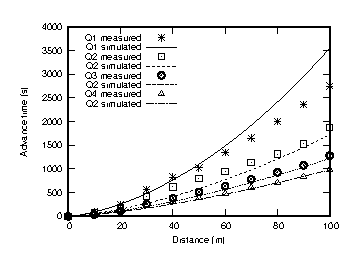
\includegraphics[width=\textwidth]{surcos-advance.eps}
\end{frame}

\begin{frame}{Furrow irrigation}
	\framesubtitle{Inlet depth evolution}
	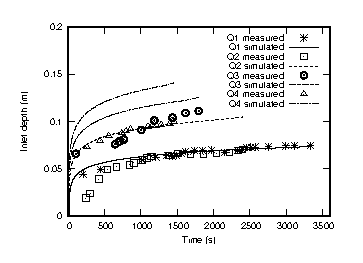
\includegraphics[width=\textwidth]{surcos-depth.eps}
\end{frame}

\begin{frame}{Furrow irrigation}
	\framesubtitle{Fertilizer concentration}
	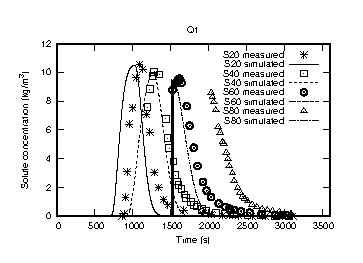
\includegraphics[width=\textwidth]{surcos-solute-q1.eps}
\end{frame}

\begin{frame}{Furrow irrigation}
	\framesubtitle{Fertilizer concentration}
	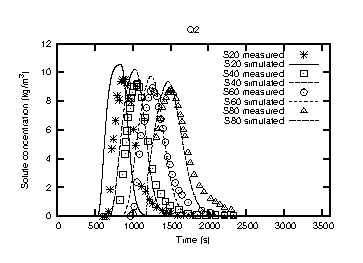
\includegraphics[width=\textwidth]{surcos-solute-q2.eps}
\end{frame}

\begin{frame}{Furrow irrigation}
	\framesubtitle{Fertilizer concentration}
	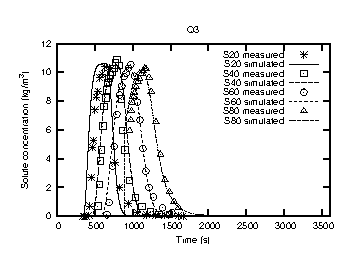
\includegraphics[width=\textwidth]{surcos-solute-q3.eps}
\end{frame}

\begin{frame}{Furrow irrigation}
	\framesubtitle{Fertilizer concentration}
	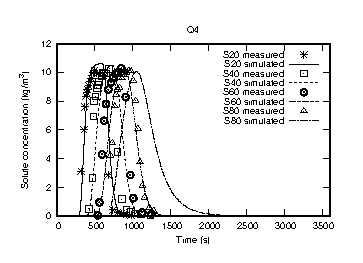
\includegraphics[width=\textwidth]{surcos-solute-q4.eps}
\end{frame}

\subsection{Calibration of size and friction coefficients in
sprinklers}

\begin{frame}
\end{frame}

\subsection{Calibration of movement coefficients in pivots}

\begin{frame}{Pivot irrigation machines movement}
	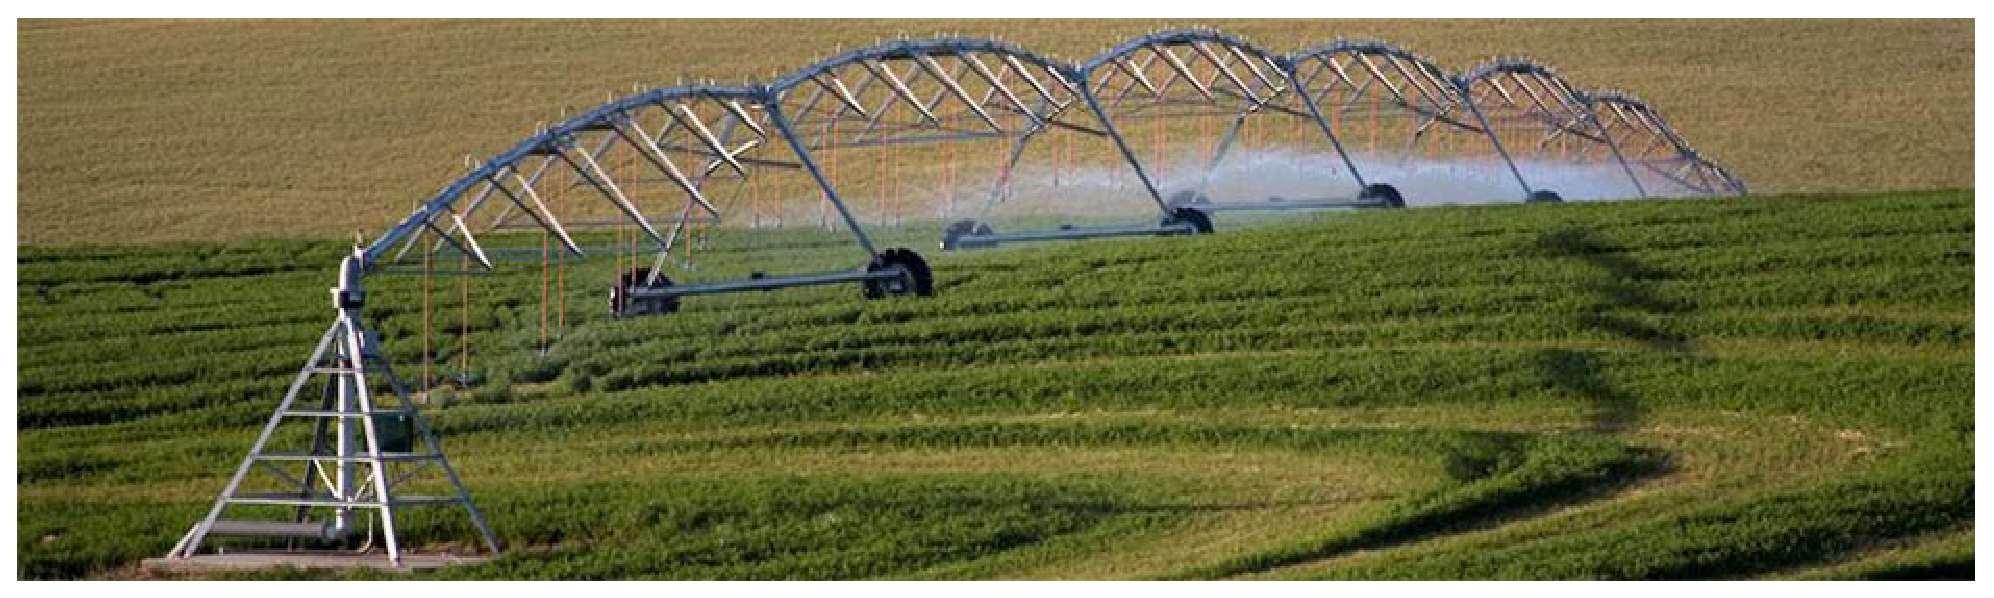
\includegraphics[width=\textwidth]{Pivot.eps}
\psset{unit=1mm}
\PSPICTURE{-10}{-6}{93}{20}
{
	\rput(25,17){$\alpha_i<\alpha_{start}\;\Rightarrow\;T_i$ start}
	\rput(65,17){$\alpha_i>\alpha_{stop}\;\Rightarrow\;T_i$ stop}
	\psarc{->}(0,0){93}{0}{7}
	\psline(0,0)(20,0)(40,1)(60,2.5)(90,5.5)
	\pscircle*(20,0){0.5}
	\pscircle*(40,1){0.5}
	\pscircle*(60,2.5){0.5}
	\pscircle*(80,4.5){0.5}
	\pscircle*(0,0){1.0}
	\rput(0,-3){Centre}
	\rput(20,-3){$T_1$}
	\rput(40,-2){$T_2$}
	\rput(60,-0.5){$T_3$}
	\rput(80,1.5){$T_4$}
	\psarc(20,0){3}{2.86}{180}
	\psarc(40,1){3}{4.29}{177.14}
	\psarc(60,2.5){3}{5.71}{175.71}
	\rput(20,6){$\alpha_1$}
	\rput(40,7){$\alpha_2$}
	\rput(60,8.5){$\alpha_3$}
}\end{frame}

\begin{frame}{Pivot irrigation machines movement}
	\framesubtitle{Tower velocity}
\psset{unit=1mm}
\PSPICTURE{-16}{-6}{75}{39}
{
	\footnotesize
	\psline{->}(0,0)(0,30)
	\psline{->}(0,0)(70,0)
	\rput(0,36){Tower}
	\rput(0,32){linear velocity}
	\rput(70,-3){Time}
	\psline(0,0)(10,0)(15,20)(25,20)(30,0)(45,0)(50,20)(60,20)(65,0)
	\rput(-8,22){Maximum}
	\rput(-8,18){velocity}
	\psline[linestyle=dotted](0,20)(15,20)
	\psline{<->}(10,23)(15,23)
	\rput(12.5,26){$\tau$}
	\psline{<->}(10,29)(30,29)
	\rput(20,35){Start}
	\rput(20,32){time}
	\psline{<->}(25,23)(30,23)
	\rput(27.5,26){$\tau$}
	\psline{<->}(30,23)(45,23)
	\rput(37.5,29){Stop}
	\rput(37.5,26){time}
}
\end{frame}

\begin{frame}{Pivot irrigation machines movement}
	\framesubtitle{Chaotic regime of starts and stops}
	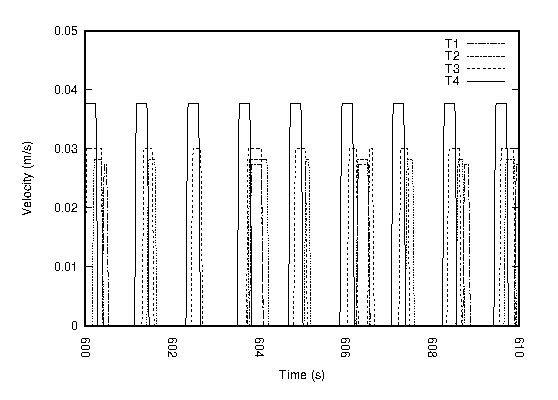
\includegraphics[width=0.9\textwidth]{pivot-velocity.eps}
\end{frame}

\begin{frame}{Pivot irrigation machines movement}
	\framesubtitle{Calibration}
	\begin{itemize}
		\item 24 hours of simulation
		\item 10000 simulations
		\item $\approx$ 50m in a laptop computer.
	\end{itemize}
\end{frame}

\begin{frame}{Pivot irrigation machines movement}
	\framesubtitle{Calibration}
\TABLE{\tiny}{cccc}
{
	Optimization & Optimization & Optimal empirical & Objective
	\\ algorithm & parameters & parameters & function value
	\\ \hline
	SW & $N_x=10$ & $\overline{\alpha_{start}}=179.956^\circ$
	& 63.03
	\\ & & $\overline{\alpha_{stop}}=180.367^\circ$
	\\ & & $\delta=0.133^\circ$
	\\ & & $\tau=1.73$ s
	\\ \hline
	SW+IT & $N_x=5$ & $\overline{\alpha_{start}}=180.448^\circ$
	& 44.30
	\\ & $N_i=16$ & $\overline{\alpha_{stop}}=180.848^\circ$
	\\ & $N_b=10$ & $\delta=0.098^\circ$
	\\ & $tol=0.5$ & $\tau=2.24$ s
	\\ \hline
	MC & $N_s=10000$
	& $\overline{\alpha_{start}}=179.739^\circ$ & 61.49
	\\ & $N_i=1$ & $\overline{\alpha_{stop}}=180.139^\circ$
	\\ & & $\delta=0.120^\circ$
	\\ & & $\tau=2.35$ s
	\\ \hline
	MC+IT & $N_s=625$
	& $\overline{\alpha_{start}}=179.760^\circ$ & 49.14
	\\ & $N_i=16$ & $\overline{\alpha_{stop}}=180.159^\circ$
	\\ & $N_b=10$ & $\delta=0.101^\circ$
	\\ & $tol=0.1$ & $\tau=2.29$ s
	\\ \hline
}
\end{frame}

\begin{frame}{Pivot irrigation machines movement}
	\framesubtitle{Calibration}
\TABLE{\tiny}{cccc}
{
	\hline
	MC+DS+CD & $N_s=9000$, $N_{st}=125$
	& $\overline{\alpha_{start}}=179.743^\circ$ & 54.42
	\\ & $rel=1$ & $\overline{\alpha_{stop}}=180.138^\circ$
	\\ & $st_{\overline{\alpha_{start}}}=0.4$ & $\delta=0.120^\circ$
	\\ & $st_{\overline{\alpha_{stop}}}=0.3$ & $\tau=2.36$ s
	\\ & $st_\delta=0.004$
	\\ & $st_\tau=0.05$
	\\ \hline
	GE & $N_p=1000$ & $\overline{\alpha_{start}}=179.967^\circ$
	& 49.41
	\\ & $N_g=16$ & $\overline{\alpha_{stop}}=180.367^\circ$
	\\ & $R_m=R_r=R_a=0.2$ & $\delta=0.101^\circ$
	\\ & & $\tau=2.22$ s
	\\ \hline
	GE & $N_p=400$ & $\overline{\alpha_{start}}=179.933^\circ$
	& 48.08
	\\ & $N_g=81$ & $\overline{\alpha_{stop}}=180.327^\circ$
	\\ & $R_m=R_r=R_a=0.1$ & $\delta=0.112^\circ$
	\\ & & $\tau=2.60$s
	\\ \hline
}
\end{frame}

\begin{frame}{Start histograms: 100\%}
	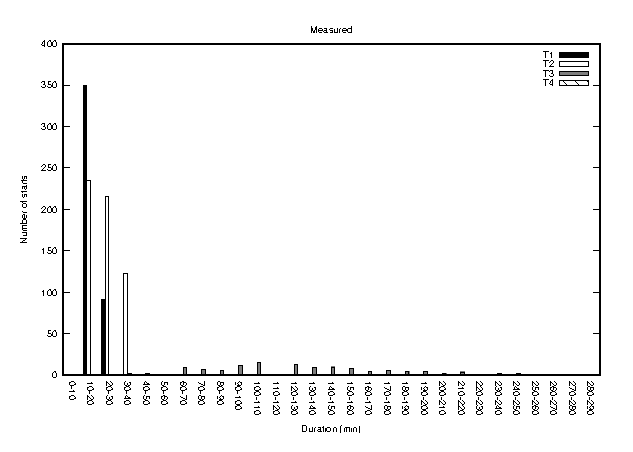
\includegraphics[width=0.60\textwidth]{pivot-measured-starts-100.eps}\\
	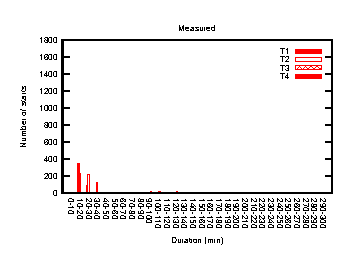
\includegraphics[width=0.60\textwidth]{pivot-simulated-starts-100.eps}
\end{frame}

\begin{frame}{Stop histograms: 100\%}
	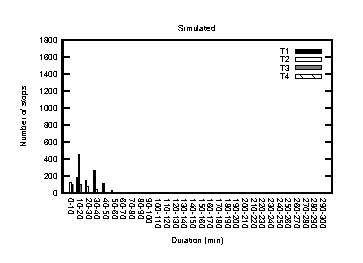
\includegraphics[width=0.60\textwidth]{pivot-measured-stops-100.eps}\\
	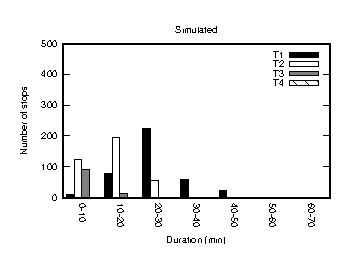
\includegraphics[width=0.60\textwidth]{pivot-simulated-stops-100.eps}
\end{frame}

\begin{frame}{Start histograms: 50\%}
	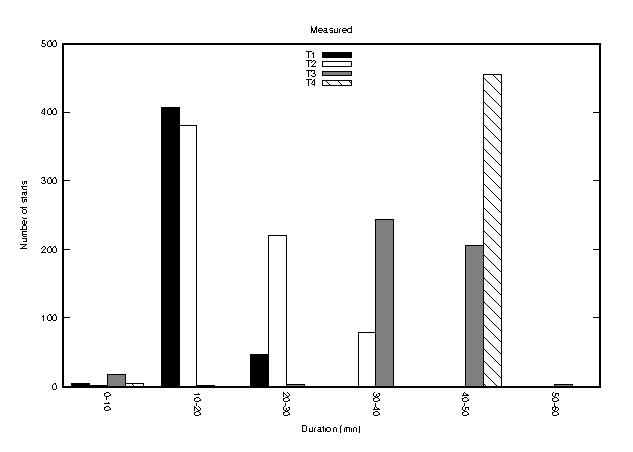
\includegraphics[width=0.60\textwidth]{pivot-measured-starts-50.eps}\\
	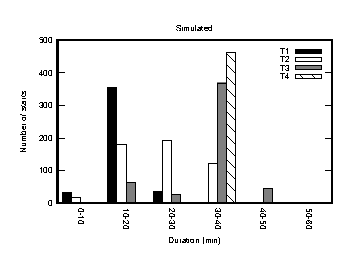
\includegraphics[width=0.60\textwidth]{pivot-simulated-starts-50.eps}
\end{frame}

\begin{frame}{Stop histograms: 50\%}
	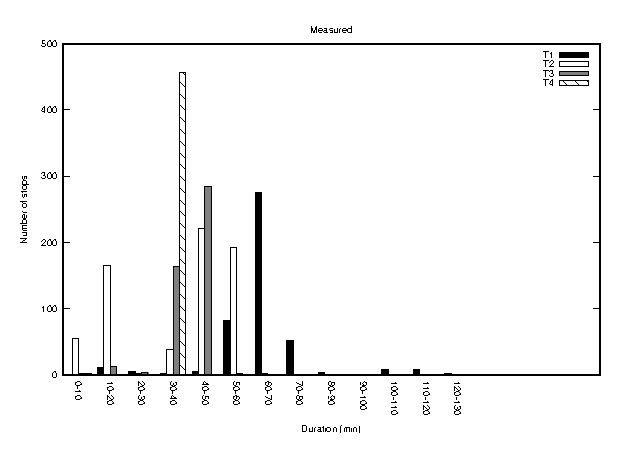
\includegraphics[width=0.60\textwidth]{pivot-measured-stops-50.eps}\\
	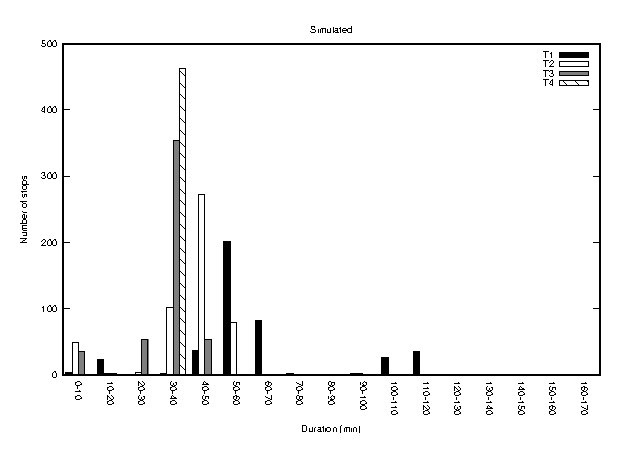
\includegraphics[width=0.60\textwidth]{pivot-simulated-stops-50.eps}
\end{frame}

\begin{frame}{Start histograms: 40\%}
	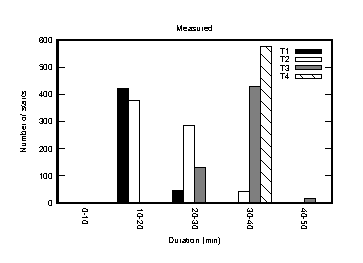
\includegraphics[width=0.60\textwidth]{pivot-measured-starts-40.eps}\\
	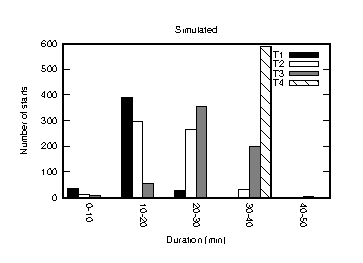
\includegraphics[width=0.60\textwidth]{pivot-simulated-starts-40.eps}
\end{frame}

\begin{frame}{Stop histograms: 40\%}
	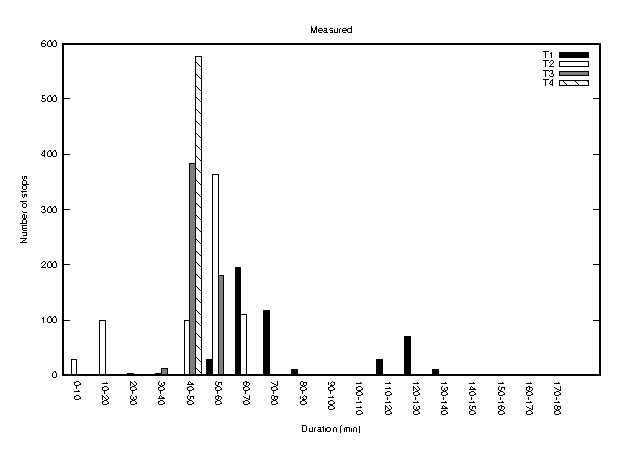
\includegraphics[width=0.60\textwidth]{pivot-measured-stops-40.eps}\\
	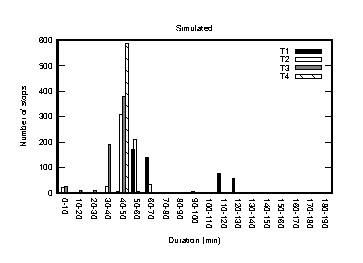
\includegraphics[width=0.60\textwidth]{pivot-simulated-stops-40.eps}
\end{frame}

\begin{frame}{Start histograms: 25\%}
	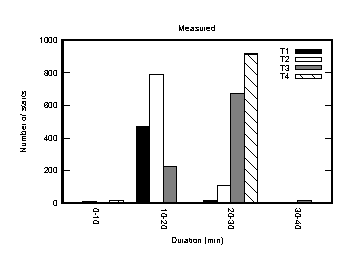
\includegraphics[width=0.60\textwidth]{pivot-measured-starts-25.eps}\\
	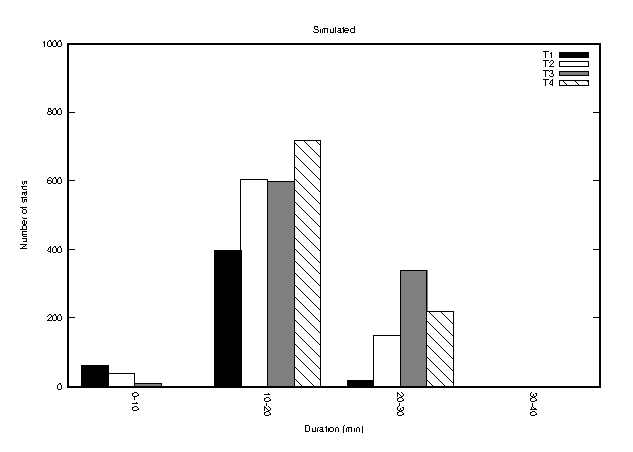
\includegraphics[width=0.60\textwidth]{pivot-simulated-starts-25.eps}
\end{frame}

\begin{frame}{Stop histograms: 25\%}
	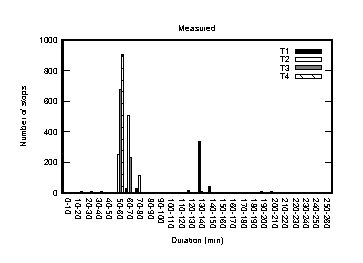
\includegraphics[width=0.60\textwidth]{pivot-measured-stops-25.eps}\\
	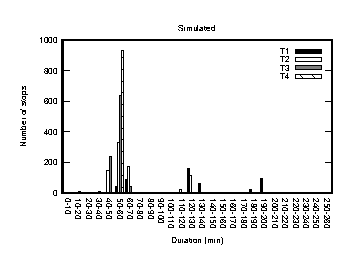
\includegraphics[width=0.60\textwidth]{pivot-simulated-stops-25.eps}
\end{frame}

\section{Conclusions}

\begin{frame}{Conclusions}
\begin{itemize}
	\item Optimization, and calibration as a particular case, is an art. Results
		depend on the shape of the objective function
	\item Practical problems in agricultural are not well conditioned to be
		calibrated/optimized
	\item MPCOTool is a easy, flexible, intuitive, robust, ..., tool for
		calibration/optimization
	\item MPCOTool implements several of the most useful general algorithms of
		optimization
	\item MPCOTool is able to use parallelized all available computational
		resources in an easy manner
	\item MPCOTool is free software with a BSD type license
\end{itemize}
\end{frame}

\begin{frame}
	\begin{center}
		\LARGE ¡GRACIAS!\\
%		\includegraphics[width=6cm]{Huerto.eps}
%		\includegraphics[width=6cm]{Vehiculo.eps}
	\end{center}
\end{frame}

\end{document}
